\documentclass[phd,tocprelim]{cornell}
\let\ifpdf\relax

\usepackage{amsmath}
\usepackage{amsthm}

%%%%%%%%%%%%%%%%%%%%%%%%%
                        %
\def\pgfsysdriver{pgfsys-dvipdfm.def}
\usepackage{caption}
%\usepackage{hangcaption}
%\usepackage{algorithmic}
%\usepackage{algorithmicx}
\usepackage{algorithm}
\usepackage{algpseudocode}
\usepackage{float}
\usepackage{ifthen}
\usepackage{soul} %For highlights
\usepackage{tikz}
\usepackage[export]{adjustbox}

%To help keep figures and tables in order:
\usepackage{fixltx2e}
%To fix quotes in verbatim, etc:
\usepackage{upquote,textcomp}

%Some possible packages to include
\usepackage{epsfig}
\usepackage{graphicx,pstricks}
\usepackage{graphics}
\usepackage{palatino}
%\usepackage{subfigure}
\usepackage{subcaption}
\usepackage{txfonts}


\graphicspath{{./figures/}}

\usetikzlibrary{shapes, arrows}

\makeatletter
\newlength{\parskipsave}
\newcommand\floatc@plainthin[2]{
\setbox\@tempboxa\hbox{{\@fs@cfont #1:} #2}
   \hbox to\hsize{\hfil\box\@tempboxa\hfil}\fi}
\newcommand\fs@plainthin{
  \def\@fs@cfont{\rmfamily}\let\@fs@capt\floatc@plainthin
  \def\@fs@pre{}
  \def\@fs@post{\vspace{-2.5em}}
  \def\@fs@mid{\vspace\abovecaptionskip\relax}
  \let\@fs@iftopcapt\iffalse}
\makeatother

\floatstyle{plainthin}
\newfloat{AlgFloat}{h}{lop}


\renewcommand{\topfraction}{0.85}
\renewcommand{\textfraction}{0.1}
\renewcommand{\floatpagefraction}{0.75}
%\renewcommand{\algorithmicrequire}{\textbf{Input:}}
%\renewcommand{\algorithmicensure}{\textbf{Output:}}
%\newcommand{\INDSTATE}[1][1]{\STATE\hspace{#1\algorithmicindent}}
\algnewcommand\algorithmicinput{\textbf{INPUT:}}
\algnewcommand\INPUT{\item[\algorithmicinput]}
\algnewcommand\algorithmicoutput{\textbf{OUTPUT:}}
\algnewcommand\OUTPUT{\item[\algorithmicoutput]}

\newtheorem{Theorem}{Theorem}
\newtheoremstyle{break}  % follow `plain` defaults but change HEADSPACE.
  {\topsep}   % ABOVESPACE
  {\topsep}   % BELOWSPACE
  {\itshape}  % BODYFONT
  {-1em}      % INDENT (empty value is the same as 0pt)
  {\bfseries} % HEADFONT
  {}         % HEADPUNCT
  {0pt}  % HEADSPACE. `plain` default: {5pt plus 1pt minus 1pt}
  {}          % CUSTOM-HEAD-SPEC
\theoremstyle{break}
\newtheorem{Algorithm}{Algorithm}

\DeclareMathOperator*{\argmin}{arg\,min}
\newcommand{\E}[1]{\operatorname{E}\left(#1\right)}
\newcommand{\sgn}[1]{\operatorname{sgn}\left(#1\right)}  %
                        %
%%%%%%%%%%%%%%%%%%%%%%%%%

%
% tocprelim option must be included to put the roman numeral pages in the
% table of contents
%
% The cornellheadings option will make headings completely consistent with
% guidelines.
%
% This sample document was originally provided by Blake Jacquot, and
% fixed up by Andrew Myers.
%
% ************* TODO (Brandon Barker) ***********************************
%
% Cool idea for last chapter: use FALCON and a MILP version of FALCON
% (compatible with LFP?) to try and estimate whole-cell-model fluxes.
%
%General
% Figure out the best way to modularize chapters/sections in different files.
%
% Verify bibliography working; check FALCON script and add to Makefile?
%
% Appendix can work as a place for supplementary notes and figures?
%
% Semi-automate Mendeley->.bib citation process
% TODO (Brandon Barker)
% Read Formatting Rules on Grad School site.
%  - referencing figures/capitalization: Fig or fig or figure ...
%
% Spellcheck
%
% Permissions: Once title of thesis is known, write permission letter to use publications
% http://www.proquest.com/assets/downloads/products/UMI_CopyrightGuide.pdf
% E-mail Wiley @ permissionsus@wiley.com
%
%
% Word histogram to check for words used too often.
%

% Chapter 1: Introduction:
% Add other (Jason-deleted) sections/words - update correct figure 1
% Refs/Figs
% Epistasis
%
% Chapter 2: Using FBA to understand epistasis dynamics.
%
% Interlude: discuss limitations of FBA for epistasis, etc (e.g. Papp, beneficial mutations).
%
% Chapter 3: FALCON
% 
% Chapter 4: MILP-FALCON/whole-cell-model
%
% Chapter 5: An improved undestanding of epistasis
%

% Consider adding the Motif/model work somehow?


%Chapter 3:
%
% Figure/table: be sure to show the differences for minDisj and
% original method on the human network, somehow.
%
% Do I discuss the issue of negative fluxes in the FALCON objective?
%
% Parameter sensitivity analysis for initial flux
% scaling value.
%
% Consider discussing ass:chap and ass:rate in the text.
% Perhaps discuss related to ass:rate that a penalty deriving
% from mass-action considerations is warranted - cite Karr2012
%
% Relatedly, discuss how how min(a,b) is a good approximation
% to mass-action assumptions -- need to think about this:
% since mass action would propose r = [a][b], then we would have
% log(r) = log(a) + log(b) ... hmm
%
%
% Discuss Assumption: complexation formation assumption (recall Tom Fox's talk)
% Discuss Assumption: Localization (Pablo Meyer, IBM):
%     http://researcher.watson.ibm.com/researcher/view.php?person=us-pmeyerr
% 
%
% Add discussion on atomic (Lee et al) versus batch direction
% assignment.
%
% Fix missing references.
%
% Tie in motivating rules example with previous section
% showing the merits of CNF
%
% Add another illustrative figure.
%
% Add a table/figure comparing estimated EC abundance using
% e.g. original method vs our method, also for fluxes.
% - Benchmark these against cancer data in Chapter 5
%
% Discuss incrementing flux_sum at each iteration.
%
% Figure out how copyright registration is handled; apparently it is necesasry.
% I assume it is handled by Cornell.
%

% ************* End of TODO ***********************************************
%Added by Brandon:
%\usepackage[amsmath,amsthm,thmmarks]{ntheorem}
\usepackage{hyperref}


%if you're having problems with overfull boxes, you may need to increase
%the tolerance to 9999
\tolerance=9999

\renewcommand{\caption}[1]{\singlespacing\hangcaption{#1}\normalspacing}

\bibliographystyle{plain}
\title {Advances in Genome-Scale Metabolic Models Applied to Adaptive and Environmental Epistatic Landscapes and Cancer Physiology}
\author {Brandon Barker}
\conferraldate {August}{2013}
\degreefield {Ph.D.}
\copyrightholder{Brandon Elam Barker}
\copyrightyear{2013}


%%%%%%%%%%%%%%%%%%
\begin{document}%%
%%%%%%%%%%%%%%%%%%

\newboolean{thesisStyle}
\setboolean{thesisStyle}{true}

%%%%%%%%%%%%%%%%%%%%%%%%%%%%
                           %
../documentHeadCommon.tex %
                           %
%%%%%%%%%%%%%%%%%%%%%%%%%%%%

\maketitle
\makecopyright

\begin{abstract}

Quantitative models are increasingly being used to interrogate the
metabolic pathways that are contained within complex biological
processes, and at a higher level, these models are used to explore
questions in population genetics with complex physiological processes
absent in typical, idealized population genetic models.  I give an
overview of constraint-based modeling and its purview in the field of
metabolic modeling. By using a simple version of constraint-based
modeling known as flux balance analysis, we elucidate patterns that
occur in gene-gene interactions of deleterious mutations and the
influences that metabolic network architecture may bring to bear on
adaptation. We then turn to developing approaches that enable the
simulation of beneficial mutations, allowing the study of effects of
different parameters on genetic interaction patterns occurring during
environmental adaptation. Because many of these approaches rely on
establishing a physiologically accurate flux for the wild-type
organism, we address the problem of estimating metabolic fluxes using
gene expression data and constraint-based models. Finally, this
methodology is employed in the separate context of cancer metabolism
analysis.
\end{abstract}

\begin{biosketch}
Your biosketch goes here. Make sure it sits inside
the brackets.
\end{biosketch}

\begin{dedication}
\begin{center}
\textit{To my parents---James and Carol Barker, \\
For their love, time, and beneficence, \\
Without which this work would not have been possible. \\
\vspace{10 mm} 
To my wife, Lin Xue, \\
For giving me the mommentum to pursue graduate school, \\
For her patience while I studied, \\
For her continuing love and , \\
And most importantly, for being an amazing mother.\\
\vspace{10 mm} 
To my son, Lindon Barker, \\
For your extra motivation towards finishing in a timely manner, \\
And for your terrific smiles, grins, and laughs during this last year.}
\end{center}
\end{dedication}

\begin{acknowledgements}
Firstly I would like to thank my advisor,  Zhenglong Gu, under
whose supervision this work has unfolded, and who has provided me with
substantial support, encouragement, and irreplacable mentoring. I owe
much to my colleague and friend, Lin Xu, for not only showing me
the ropes and giving me hope, but also getting me interested in so
many topics in evolution; much of the present work, particularly that
involving epistasis, would not have happened without him. Without
Jason Locasale's intellectual incitation and advise, I never would
have wandered down the path to what has, to me, become the most
interesting part of this work, nor the path to the Big Red Barn quite
so much as I did. My thesis committee members---David Christini,
Chris Myers, and Michael Stillman---have provided much advice
over the years, scientific and otherwise.

My other collaborators in the present work include Tim Connallon,
whose knowledge on epistasis surpasses anyone I know, and similarly
for Alex Shestov with regard to metabolic flux analysis;
Kieran Smallbone, who has given helpful advice over the years 
regarding constraint-based models, as well as having helped develop several  
algorithms and models that I have employed in this work, including one in 
particular that served as the impetus for some of the research in the latter 
chapters; Yiping Wang, a phenomenal young researcher who helped
with some analysis in the last chapter during his first month on
campus, and Hongwei Xi, for providing substantial support for his
programming language ATS, which was employed in the latter chapters.

In the lab, Xiaoxian Guo, Huifeng Jiang, and Zhe Wang
provided much experimental advice, training, and data.

I would also like to thank many other colleagues for their help,
friendship, scientific discussion, or some combination of
the three. These include Diana Chang, Elijah Bogart, 
Hong Chian, Martha Field, Lei Huang,
Haley Hunter-Zinck, Ben Heavner, Xiaojing Liu, Henry Lu, Anuttama Mohan,
Lonnie Princehouse, Narayanan Sadagopan, and Kaixiong Ye.

Without the stimulus, confidence, and aid from my early mentors at the
University of Kentucky, this document would not exist; in particular,
I thank Ruriko Yoshida, for renewing my passion in science,
Jim Lund, for being my first biology mentor (and providing the
opportunity to become acquainted with my wife), Jerzy Jaromczyk
for his friendly help and advice throughout and beyond my
undergraduate education, and to Henry Dietz, for being a great
educator and advising my senior design project.  My passionate and
reassuring high school biology teacher, David Christiansen,
warrants special thanks for being continually amazed at the wonders
biology has to offer. Lastly, I thank my friend Benjamin Runyon,
for always lending an ear.
\end{acknowledgements}

\contentspage
\tablelistpage
\figurelistpage

\normalspacing \setcounter{page}{1} \pagenumbering{arabic}
\pagestyle{cornell} \addtolength{\parskip}{0.5\baselineskip}

\chapter{Introduction}

There has been a surge of interest in understanding the regulation of
metabolic networks involved in disease in recent years.  Quantitative
models are increasingly being used to interrogate the metabolic
pathways that are contained within this complex disease biology.  At
the core of this effort is the mathematical modeling of central carbon
metabolism involving glycolysis and the citric acid cycle (referred to
as energy metabolism).  Here we discuss several approaches used to
quantitatively model metabolic pathways relating to energy metabolism
and discuss their formalisms, successes, and limitations.  Your
abstract goes here. Make sure it sits inside the brackets. If not,
your biosketch page may not be roman numeral iii, as required by the
graduate school.

The accumulated amount of biochemical work carried out over the years
has elaborated complex metabolic systems and networks.  This
information includes the network architecture encoded in chemical
reactions that are carried out by metabolic enzymes and the kinetic
parameters that determine reaction mechanisms involved in each of
these chemical reactions.  Application of this knowledge has led to
tremendous predictive capability in characterizing metabolic
regulation in normal physiology including the growth of unicellular
organisms and the successful simulation of energy metabolism in
healthy red blood cells.  However, there are far fewer instances in
which these models have been applied to the characterization of
pathophysiology.  Applying our knowledge of metabolic regulation to
the investigation of disease states such as cancer or
neurodegeneration is currently a scientific frontier.  In this review,
we will revisit several classic techniques for the mathematical
modeling of metabolic pathways and discuss instances where their
application to biomedical science is beginning to yield fruitful
dividends.

\section{Linear Systems, Flux Balance Analysis}
Linear models are mathematical models that containt a set of algebraic
equations based on the stoichiometric relationships that define
conservation relationships within a metabolic network.  Linear models,
to our knowledge, were first applied to biochemical systems in 1961 by
Howard Shapiro1. Shapiro discussed the possibility of using
optimization in biochemical linear models in a 1969 publication2. In
1984, a model incorporating glycolysis and the TCA cycle was employed
running a variant of Dantzig’s algorithm with the assumed biological
objective of minimized free energy dissipation3,4. An enduring
research program was initiated by Bernhard Palsson half a decade
later5,6.  An early work of Palsson showed that growth maximization in
an E. coli model could correctly match 86\% of 79 gene essentialities
examined7. Subsequent modeling in S. cerevisiae was able to closely
predict growth rates and exometabolic fluxes in various media, and
nearly capture the in vivo phosphate/oxygen (P/O) ratio of 0.94 with a
simulated P/O value of 1.04, showing that models of eukaryotes were
also feasible8. If one chooses the biological objective function to
reflect the appropriate physiological demands then it is possible to
predict features of adaptation; this was shown to be the case for
growth optimization in several E. coli mutants9. By this time it had
become apparent that linear models held much promise, particularly
when coupled with optimization.


\section{Genome Scale Modeling}
Today, when we refer to linear models, we most often mean Constraint
Based Models (CBMs). We refer to a CBM as any model making use of the
stoichiometric matrix, S, as a linear matrix constraint, e.g. S * F =
0, where F is a flux vector. In fact, this is a nearly universal
constraint, as it guarantees conservation of mass during steady state
processes such as exponential growth or tissue maintenance10. Other
constraints commonly used include reversibility constraints when the
direction of a reaction is known for physiological conditions of
interest, bounds on the uptake of nutrients or efflux rates due to
regulation or physiology, or bounds on enzyme reactions when the
maximum enzyme velocity Vmax is known.

Because these constraints give rise to an underdetermined system, it
will not be possible to identify a unique solution for the flux
vector. A unique solution is often desirable as it allows
investigators to analyze a putative metabolic phenotype. Indeed, this
is one of the more convenient features of linear optimization: the
ability to get meaningful solutions without explicitly taking into
account any, or at least very few, free parameters.  Flux Balance
Analysis, or FBA, assumes a linear combination of fluxes to be
maximized or minimized (Fig 1). In microbes, perhaps the most popular
FBA objective has been growth maximization, which consists of the
biomass precursors and products formulated as a single
pseudo-reaction. Additionally, an ATP maintenance constraint should be
formulated as a sink reaction with the molar ATP required to keep one
gram of dry weight biomass living for one hour11. This empirically
determined constraint, although assumed, is less discussed, perhaps
due to its dependence on individual strains and environments.  We note
that for many expression-based methods in the CBM framework, the ATP
maintenance constraint is not required (see Table and Fig 2 for
examples). Fixed biomass objectives by themselves also have some
undesirable qualities; biomass composition likely has some measure of
variability based on genetic background and environment.  Robust FBA
attempts to address this problem by allowing some variation in the
biomass composition, as determined by variation of empirical assays of
biomass 12.  Despite these caveats, FBA has recently been found to not
only predict growth in microbes, but also has good agreement with gold
standard 13C flux assays in vivo when the growth objective is used
along with ATP synthesis maximization and minimization of absolute
fluxes13.

Minimization of absolute flux is a commonly used objective employed
alongside other objectives, forming a minimax problem (i.e. finding
the minimum absolute flux profile among all flux profiles that
maximize biomass). This approximates the biological goal of being
efficient with enzyme production costs and enzyme crowding constraints
while also guaranteeing that no thermodynamically impossible loops are
present, that is, ruling out some fluxes that might otherwise violate
Kirchoff’s loop rule14,15.  This constraint will work whenever a sink
reaction, such as growth, is being optimized.  However, maximizing an
internal flux, as in Flux Variability Analysis16, could still result
in internal cycles15. Initial thermodynamic approaches involved
nonlinear optimization17–20.  Constraints satisfying Kirchoff’s loop
rule were later developed that were faster and more generally
applicable than prior methods15,21.  Still, these involve integer
constraints that put this problem in a slower class of algorithms than
the convex minimized absolute flux problem.  When available,
thermodynamic data is valuable; it can not only be used to guarantee
there are no internal cycles, but can also aid in determining reaction
direction and potential regulatory targets15,18,22,23. Application of
this framework to concentration data allows unmeasured metabolite
concentrations to be inferred and global concentrations to be resolved
at the organelle level20. CBMs have also found use in tracing
individual atoms through pathways, which provides a more appealing
framework for performing Metabolic Flux Analysis (MFA; discussed
below) on stable isotope data due to the lack of bias compared to
typical MFA models, which are often an order of magnitude smaller than
genome-scale reconstructions24.  Recent insightful work has made it
possible to simplify the computational complexity of loopless FBA to
be nearly the same as conventional FBA, but some mathematical
difficulties must still be overcome before bounds on exchange fluxes
can be suitably incorporated for genome-scale modeling10,25.


The metabolism of different tissues within the same organism is
diverse; whereas the metabolism in liver is anabolic, neurons or red
blood cells have a much more limited catabolic regime26–28.The
creation of tissue specific models for multicellular organism has
become an important problem, and several automated algorithms taking
as inputs tissue expression data and a generic model for the organism
have been developed28–30. Coupling multiple cellular models together
will enable multi-scale modeling of tissues in multicellular models or
entire ecosystems for microbes26,31–33.

Automated generation of metabolic networks from genome sequence and
pathway databases, especially in prokaryotes, has been developed34–37.
This will offer many advantages to modelers: a starting point for
curated models (a draft reconstruction is estimated to often take
several months even in prokaryotes), a means for doing population or
ecological simulation33, and personalized genomic modeling for
patients with metabolic syndromes such as cancer where both the
patient and possibly the disease have diverse genotypes38,39.
Eukaryotic models are somewhat more difficult to generate due to the
necessity of protein localization and metabolite transporter
information34. Automatic reconstruction going beyond enzymatic gene
information, such as rFBA models, should also be possible40,41; the
automated generation of Boolean and higher-order discrete regulatory
models using time-series expression data has been explored as well,
though to date these regulatory models have not been coupled to
metabolic reconstructions42–45. These approaches and other families of
genome-scale methods are discussed in Table 1.

Several approaches have been used in applying CBMs to cancer and the
Warburg effect, the preference for glycolytic ATP production over
glucose-derived mitochondrial ATP production in cancer cells46–48. An
important study working with a simplified, small model of
central-carbon metabolism showed that, while the TCA cycle predicts
better ATP yield than glycolysis when only available glucose is
considered as a constraint, the addition of enzyme solvent-capacity
constraints creates a preference for ATP synthesis through
glycolysis48. More recently, the work of Vazquez et al. was extended
to include a genome-scale model along with enzyme solvent-capacity
constraints, which was able to show significant correlations between
fluxes and expression in the NCI-60 cell line panel, as well as
predicting an intermediate state in cancer metabolism transition
exhibiting a temporary increase in OxPhos that was supported by two
prior experimental observations47. All of these approaches correctly
predicted lactate production. Concurrent research on predicting cancer
targets by screening for simulated negative epistasis in cancer
tissue-specific models that have at least one known-drug target and no
known effect on normal tissue revealed many epistatic
interactions39. A related study confirmed one of these synthetic
lethalities between hemeoxygenase and fumarate hydratase, a mutation
found in certain kidney cancers49. The recent publication of Human
Recon 2 promises to aid in the understanding of many human diseases;
already 65 cell-type specific models based on it are available, and
the model reports 77\% accuracy in identifying metabolic markers
across 49 inborn errors of metabolism50. Although this model is a
great step forward in consolidating much of the knowledge about human
metabolism, it is only one of many steps to come. For instance, this
model is still primarily only amenable to steady-state approaches,
lacks corresponding enzyme-regulatory and signaling architecture, and
has introduced more dead-end metabolites than it removed (1,176 versus
339). 

\section{Conclusions for the State of Linear and Genome-Scale Models}
Kinetic models for smaller pathways are possible when the data are
present, but many energetic questions concern the entire cell, leaving
only incorporation of CBMs as a viable option. The original efficiency
and ease of use of FBA have helped propagate a field of more diverse
algorithms that are often tractable on today’s computers using the
same modeling and software frameworks51,52.  Numerous methods and
successful applications in energy metabolism exist, including
prevalent diseases such as heart disease, cancer, and Alzheimer’s53.

Multiscale models, as were used in the Alzheimer’s models, will
undoubtedly become more common. At the intracellular scale, CBMs are
also beginning to incorporate information other than metabolic
stoichiometry54–56. A whole cell model for Mycoplasma genitalium
incorporating information about all classes of macromolecular
synthesis and degradation, in addition to stoichiometric and
regulatory information, found a non-stochastic coupling between
metabolism and the cell-cycle where DNA replication rates depended on
the concentration of dNTP55. Models like these are not easy to build,
but substantial endeavors are underway to assist in their draft
construction and refinement, and together with an increase in use of
jamboree meetings of organism and model experts and online
collaborative tools, will likely aid in creating public models of
higher quality and the understanding of many biological processes
outside the traditional scope of metabolism 35,50,57–61.


%\begin{equation}
%k_1=\frac{\omega }{c({1/\varepsilon_m + 1/\varepsilon_i})^{1/2}}=k_2=\frac{\omega
%sin(\theta)\varepsilon_{air}^{1/2}}{c}
%\end{equation}
%
%\noindent
%where $\omega$ is the frequency of the plasmon, $c$ is the speed of
%light, $\varepsilon_m$ is the dielectric constant of the metal,
%$\varepsilon_i$ is the dielectric constant of neighboring insulator,
%and $\varepsilon_{air}$ is the dielectric constant of air.

\chapter{Dynamic Epistasis Under Varying Environmental Perturbations}

\section{The Black Kitten}
  One thing was certain, that the WHITE kitten had had nothing to
do with it:---it was the black kitten's fault entirely~\cite{bennett2010}.  For the
white kitten had been having its face washed by the old cat for
the last quarter of an hour (and bearing it pretty well,
considering); so you see that it COULDN'T have had any hand in
the mischief.

  The way Dinah washed her children's faces was this:  first she
held the poor thing down by its ear with one paw, and then with
the other paw she rubbed its face all over, the wrong way,
beginning at the nose:  and just now, as I said, she was hard at
work on the white kitten, which was lying quite still and trying
to purr---no doubt feeling that it was all meant for its good.

  But the black kitten had been finished with earlier in the
afternoon, and so, while Alice was sitting curled up in a corner
of the great arm-chair, half talking to herself and half asleep,
the kitten had been having a grand game of romps with the ball of
worsted Alice had been trying to wind up, and had been rolling it
up and down till it had all come undone again; and there it was,
spread over the hearth-rug, all knots and tangles, with the
kitten running after its own tail in the middle.

\section{The Reproach}

  `Oh, you wicked little thing!' cried Alice, catching up the
kitten, and giving it a little kiss to make it understand that it
was in disgrace.  `Really, Dinah ought to have taught you better
manners!  You OUGHT, Dinah, you know you ought!' she added,
looking reproachfully at the old cat, and speaking in as cross a
voice as she could manage---and then she scrambled back into the
arm-chair, taking the kitten and the worsted with her, and began
winding up the ball again.  But she didn't get on very fast, as
she was talking all the time, sometimes to the kitten, and
sometimes to herself.  Kitty sat very demurely on her knee,
pretending to watch the progress of the winding, and now and then
putting out one paw and gently touching the ball, as if it would
be glad to help, if it might.

  `Do you know what to-morrow is, Kitty?' Alice began.  `You'd
have guessed if you'd been up in the window with me---only Dinah
was making you tidy, so you couldn't.  I was watching the boys
getting in stick for the bonfire---and it wants plenty of
sticks, Kitty!  Only it got so cold, and it snowed so, they had
to leave off.  Never mind, Kitty, we'll go and see the bonfire
to-morrow.'  Here Alice wound two or three turns of the worsted
round the kitten's neck, just to see how it would look:  this led
to a scramble, in which the ball rolled down upon the floor, and
yards and yards of it got unwound again.

  `Do you know, I was so angry, Kitty,' Alice went on as soon as
they were comfortably settled again, `when I saw all the mischief
you had been doing, I was very nearly opening the window, and
putting you out into the snow!  And you'd have deserved it, you
little mischievous darling!  What have you got to say for
yourself?  Now don't interrupt me!' she went on, holding up one
finger.  `I'm going to tell you all your faults.  Number one:
you squeaked twice while Dinah was washing your face this
morning.  Now you can't deny it, Kitty:  I heard you!  What that
you say?' (pretending that the kitten was speaking.)  `Her paw
went into your eye?  Well, that's YOUR fault, for keeping your
eyes open---if you'd shut them tight up, it wouldn't have
happened.  Now don't make any more excuses, but listen!  Number
two:  you pulled Snowdrop away by the tail just as I had put down
the saucer of milk before her!  What, you were thirsty, were you?

\chapter{Epistasis Landscapes Arising From Adaptive Mutations}
The literature so far has been remarkably biased in the simulation of only
deleterious mutants rather than beneficial mutants in the constraint-based modeling
literature. This has numerous reasons, but it is undoubtedly due largely to 
the absence of a notion of any improvement in the objecitve function when a global optimum
is found. 

\section{Introduction to Adaptive Mutations}
Biologists have long wondered the extent to which evolution occurs due to nearly neutral 
and slighly deleterious mutations, or adaptive mutations, or more complex situations involving
these types of mutations as well as their epistatic interactions (cite the work of Kimura etc.).
 
\subsection{Adaptive Mutations and Epistasis}

\subsection{The Need for a New Modeling Framework}
Clearly, using FBA with the growth objective alone is not enough--we only ever get the 
optimum for our fitness objective.

\chapter{FALCON: Flux Assignment (with) LAD Convex Objectives}

\falconAbstractMotivation \falconAbstractResults

%%%%%%%%%%%%%%%%%%%
%                 %
\section{Introduction}

%
% Thanks to Martha Field for discussion on adapting mammalian cells
% to synthetic media.
%
FBA has become extremely popular, in part, due to its simplicity in
calculating reasonably accurate microbial fluxes. For many microbes, a
simple synthetic environment where all chemical species are known
suffices to allow proliferation. Additionally, it has been found that
their biological objectives can be largely expressed as linear
objectives of fluxes.  Neither of these assumptions necessarily hold
for mammalian cells growing \emph{in vitro} or \emph{in vivo}, and in
particular the environment is far more complex for mammalian cell
cultures, which have to undergo gradual metabolic adaptation via
titration to grow on synthetic media. In what follows we first discuss
the MoMA algorithm since it is heavily extended in order to allow us
to use expression data for the estimation of flux data.

% May eventually want to make this a conditional include section
% and include it earlier in dissertation.
\subsection{MoMA: Minimization of Metabolic Adjustment}

The minimization of metabolic adjustment (MoMA) method
\citep{Segre2002}, which is framed as a least-squares optimization
problem, is typically employed to calculate the flux vector of an
\emph{in silico} organism after a mutation by minimizing the distance
between the wild-type flux and the mutant flux. The biological
intuition is that the organism has not had time to adapt to the
restricted metabolic capacity and will maintain a similar flux to the
wild-type (WT) except where the perturbations due to the mutation
dictate necessary alterations in fluxes \citep{Shlomi2005}.

Suppose $\mathbf{a}$ is the WT flux vector obtained by an optimization
procedure, such as min-norm FBA (flux balance analysis), empirical
measurements, or a combination of these. Then for an undetermined flux
vector $\mathbf{v}$ in a model with $N$ reactions the optimization
objective can be expressed as
\[ \textnormal{minimize}\ \sum\limits_{i=1}^N (v_i-a_i)^2 \] subject to the
stoichiometric constraints $\mathbf{S v} = \mathbf{0}$ where
$\mathbf{v} = (v_1, \ldots, v_N)^T$. This assumes that each $a_i$ is
measured, but it is also possible and sometimes even more useful to
employ this objective when only a subset of the $a_i$ are measured (if
$a_i$ is not measured for some $i$, then we omit $(v_i-a_i)^2$ from
the objective). In metabolomics, for instance, it is always the case
in experiments with labeled isotope tracers that only a relatively
small subset of all fluxes are able to be estimated with metabolic
flux analysis (MFA). Combining MoMA with MFA provides a technique to
potentially estimate other fluxes in the network.  Constant bounds on
fluxes are often present, such as substrate uptake limits, or
experimental $v_{max}$ estimates, so we write these as the constraints
$\mathbf{v}_{lb} \preceq \mathbf{v} \preceq \mathbf{v}_{ub}$.

The objective may be equivalently expressed in the canonical quadratic
programming (QP) form as

\[ \textnormal{minimize}\ \frac{1}{2}\mathbf{v}^T \mathbf{v} -
\mathbf{a}^T \mathbf{v}\textnormal{.}\]

A variant of MoMA exists that minimizes the absolute value of the
difference between $a_i$ and $v_i$ for all known $a_i$. To our
knowledge, the following linear program is the simplest version of
linear MoMA, which assumes the existence of a constant flux vector
$\mathbf{a}$ and is expressed as the following linear program:

\begin{align*}
&\textnormal{minimize}\ \sum\limits_{i=1}^N d_i  \\
&s.t.\\
&\mathbf{S v} = \mathbf{0} \\
&\mathbf{v}_{lb} \preceq \mathbf{v} \preceq \mathbf{v}_{ub} \\
\forall i:~~&-d_i \le v_i-a_i \le d_i \\
&d_i \ge 0
\end{align*}

The $d_i$ have no physical meaning and are minimized to force model
fluxes to be as close as possible to the measured flux.  Linear MoMA
has the advantage that it is not biased towards penalizing large
magnitude fluxes or conversely under-penalizing fluxes that are less
than one. Additionally, linear programs are often amenable to more
changes that maintain convexity than a quadratic program.

\section{Methods}

If we wish to apply MoMA to expression data rather than flux data, the
original MoMA objective must be altered in several ways. Scaling of
expression values must be addressed so they can be comparable to
fluxes in the minimization. Also, expression data has no
directionality, so a method to determine reaction direction given the
model and expression data must be devised. Prior work that served as
an inspiration for this method used Flux Variability Analysis (FVA) to
determine reaction direction \citep{Lee2012}. Briefly, this involves
two FBA simulations per reaction catalyzed by an enzyme, and as the
algorithm is iterative, this global (and costly) procedure may be run
several times before converging to a flux vector. We term any
MoMA-like algorithm applied to expression data as FALCON. To our
knowledge, there are only two such algorithms including the present
work \citep{Lee2012}.

Most genome-scale models have attached Boolean gene rules (without
negation) to aid in determining whether or not a gene deletion will
completely disable a reaction. These are typically called GPR
(gene-protein-reaction) rules and are a requirement for FALCON; their
validity, like the stoichiometric matrix, will undoubtedly be
important for generating accurate predictions. Also important are the
assumptions and limitations for the process of mapping expression data
to complexes. We address these in the next section and have attached a
flow chart to illustrate the overall process of mapping expression of
individual genes to enzyme complexes (figure~\ref{ECCN_flowchart}).

\vspace{5 mm} 
\begin{figure}
\begin{center}
\begin{tikzpicture}%[scale=0.8, node distance = 1cm, auto]
    % Place nodes
    \node [block] (start) {start}; 
    \node [iogram, below of=start, left of=start] (exp) {Gene: 
      $\mu$,~$\sigma^2$}; 
    \node [iogram, below of=start, right of=start] (rules) {Reaction:
      Gene Rule}; 
    \node [block, below of=rules] (parse) {Parse Rule}; 
    \node [block, below of=parse, left of=parse, xshift=-0.5cm]
      (mindisj) {Find minimum disjunction};
    \node [iogram, below of=mindisj] (expstd)
          {Reaction\\(enzyme~complex): $\mu$,~$\sigma^2$};
    % Draw edges
    \path [line] (start) -- (exp);
    \path [line] (start) -- (rules);
    \path [line] (rules) -- (parse);
    \path [line] (exp.south) -- (mindisj);
    \path [line] (parse) -- (mindisj);
    \path [line] (mindisj) -- (expstd);
\end{tikzpicture}
\end{center}
\caption{Flowchart illustrating the process of estimating enzyme
  complex copy number. First, for each gene in the model with
  available expression data, the mean and (if available) variance or
  some other measure of uncertainty are read in. Gene rules (also
  called GPR rules) are also read in for each enzymatic reaction. The
  reaction rules are parsed and the minimum disjunction algorithm
  (Algorithm~\ref{alg:ReductionToCNF}) is applied, making use of the
  gene's mean expression. Finally, the estimated and unitless enzyme
  complex copy number and variance are output for each enzymatic
  reaction.}
\label{ECCN_flowchart}
\end{figure}

The last step, \emph{Find Min. Disjunction} is an algorithm we have
developed to estimate the expression as accurately as possible given
the assumptions that are elaborated in the next section.

\subsection{A Formalism for Enzyme Complex Formation}

Given the abundance of genome-scale expression datasets available,
either as microarray or more recently RNA-Seq, it could be useful to
actually gauge the number of enzyme complexes present in a cell. This
isn't much of an issue for the simplest case where a reaction is
catalyzed by only one polypeptide, and that polypeptide does not
catalyze any other reactions.  Frequently the situation is not so
simple (e.g. figure~\ref{fig:2F43}), so a model of enzyme complex
formation is called for.  We formalize such a model for enzyme complex
formation based on GPR (gene-protein-reaction) rules that are
frequently available in genome-scale annotations. For better curated
models, the approach described immediately finds use for understanding
metabolism, as well as being a scaffold to find problems for existing
GPRs, and more broadly the GPR formalism itself.

\subsubsection{Assumptions for Enzyme Complex Formation}
\emph{Assumption~\ref{asm:expcorr}.}
The first assumption that we need in order to guarantee an accurate
estimate of (relative) enzyme complex copy number are accurate
measurements of their component subunits. Unfortunately, this is
currently not possible, and we almost always must make do with mRNA
measurements, which may even have some degree of inaccuracy in
measuring the mRNA copy number. What has been seen is that Spearman's
$\rho = 0.6$ for correlation between RNA-Seq and protein inensity in
datasets from HeLa cells \citep{Nagaraj2011}. This implies that much
can likely still be gleamed from analyzing RNA-Seq data, but, an
appropriate degree of caution must be used in interpreting results
based on RNA-Seq data. By incorporating more information, such as
metabolic constaints, we hope to obviate some of the error in
estimating protein intensity from RNA-Seq data. 

\emph{Assumption~\ref{asm:isozyme}.}
In order to quantify enzyme complex formation, the notion of an enzyme
complex should be formalized.
A protein complex typically refers to two or more physically associated polypeptide chains, which is
sometimes called a quaternary structure. Since we
are not exclusively dealing with multiprotein complexes, we refer to an enzyme complex as being
one or more polypeptide chains that act together to carry out metabolic catalysis. Also, to simply
our English, we also include the notion of isozymes--different proteins that catalyze the 
same reaction--in our notion of enzyme complex. Isozymes may arise by having one or more differing
protein isoforms, and even though these isoforms may not be present in the same complex at the same
moment, we consider them to be part of the enzyme complex since one could be substituted for the other.

As an example, take the $F_1$ subcomplex of ATP Synthase (figure
~\ref{fig:2F43}), which is composed of seven protein subunits
(distinguised by color, left). On the right-hand side we see different
isoforms depicted as different colors.  Error in expression data
aside, instead of considering the copy numbers with multiplicity and
dividing their expression values by their multiplicity, it may be
easier to simply note that the axle peptide (shown in red in the
center of the complex) only has one copy in the complex, so its
expression should be an overall good estimation of the $F_1$ subcomplex
copy number. This reasoning will be useful later in considering why
GPRs may be largely adequate for estimating the abundance of most
enzyme complexes.

\begin{figure*}%[H]
\label{fig:2F43}
\centering
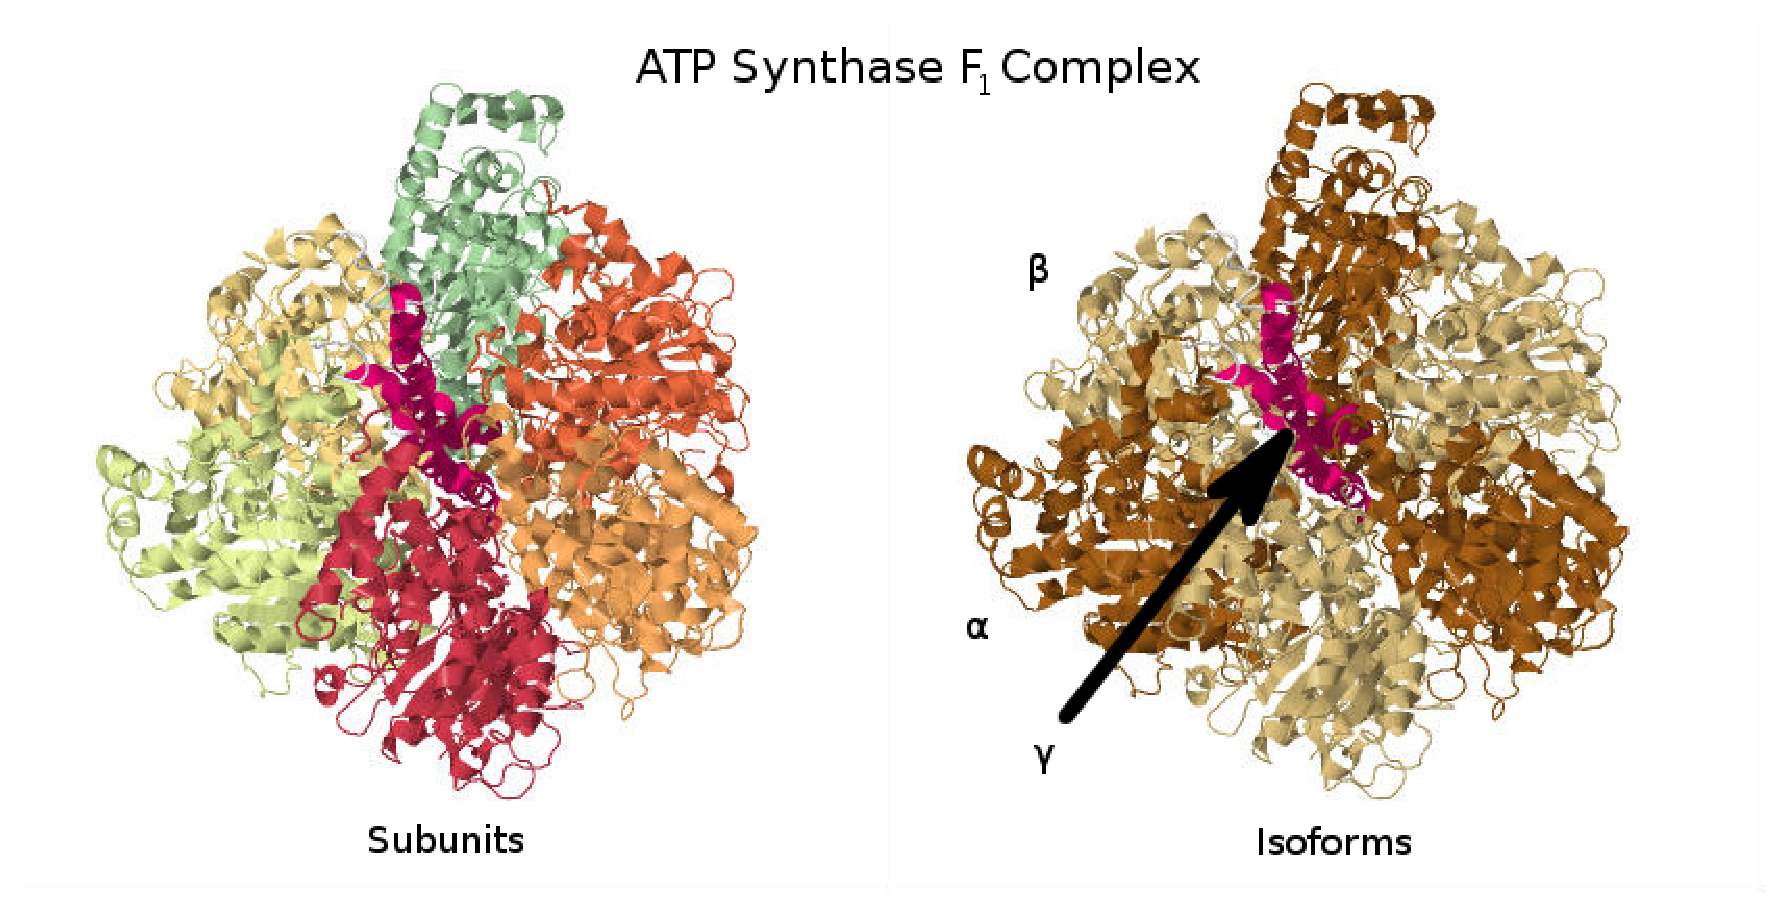
\includegraphics[clip=true,trim=0cm 0cm 0cm 0cm, width=12cm]{2F43}
\caption{Illustration of the $F_1$ part of the ATP Synthase complex
  (PDB ID 1E79; \citet{Gibbons2000,Bernstein1978,Gezelter}).
  This illustration demonstrates both how an enzyme complex may be
  constituted by multiple subunits (left), and how some of those
  subunits may be products of the same gene and have differing
  stoichiometries within the complex (right).}
\end{figure*}

\emph{Assumption~\ref{asm:hierarchy}.}
The original expression to complex-intensity mapping procedure
performed a direct evaluation of gene rule expression
values---replacing gene names with their expression values, ANDs with
minimums, and ORs with sums, without altering the logical expression
of the GPR rule in any way---can lead to problems in some
cases~\citep{Lee2012}. We illustrate this below; lower case letters
denote expression level (i.e. copy number of mRNA) of their
corresponding upper case letter, which denotes the gene name. The
$r_i$ are different reaction rules and the $e_i$ are the corresponding
estimated complex expression levels.

We need some way to guarantee that we don’t count anything twice or
more across disjunctions: 
\begin{AlgFloat}[H]
{\setlength{\tabcolsep}{.16667em}
\begin{tabular}{cccccccc}
& $r_1$ & := & [A and B] or [A and C] & $\rightarrow$ & $e_1$  &=& min($a,b$) + min($a,c$) \\ 
& $r_2$ & := & [A and (B or C)]       & $\rightarrow$ & $e_2$  &=&  min($a, b + c$) 
\end{tabular} 
}
\end{AlgFloat}
%Really we should be testing for number of text columns:
%\ifthenelse{\boolean{thesisStyle}}{\ruleEx1}{\hspace*{-4em}{\ruleEx1}} 

Supposing A is the minimum, then if we just evaluate $r_1$ directly (a
rule in disjunctive normal form, or DNF), A will be counted twice.

Another possibility is divvying up expression for a rule in DNF. For
instance, in $r_1$ above, we could evaluate it as $e_1$ =
min($\frac{a}{2},b$) + min($\frac{a}{2},c$) to account for the
repeated use of $a$. However, other potential issues aside, we can see
that this can cause problems rather quickly. For instance, suppose $b
= a$ and $c = 0$; then min($a$,$b+c$) $=b=a$ appears to be correct,
not min($\frac{a}{2},b$) + min($\frac{a}{2},c$) = $\frac{a}{2} + 0$.

The modeling of enzyme complex copy number can be tackled by using
nested sets of subcomplexes; each enzyme complex consists of multiple
subcomplexes, unlesss it is only a single protein or family of protein
isozymes.  These subcomplexes are required for the enzyme complex to
function (AND relationships), and can be thought of as the division of
the complex in to distinct units that each have some necessary
function for the complex, with the exception that we do not keep track
of the multiplicity of subcomplexes within a complex since this
information is, in the current state of affairs, not always known.
However, there may be alternative versions of each functional set
(given by OR relationships). Eventually, this nested embedding
terminates with a single protein or set of peptide isoforms
(e.g. isozymes).  In the case of ATP Synthase, one of its functional
sets is represented by the $F_1$ subcomplex. The $F_1$ subcomplex
itself can be viewed as having two immediate subcomplexes: the single
$\gamma$ (axle) subunit and three identical subcomplexes each made of
an $\alpha$ and $\beta$ subunit. Each $\alpha\beta$ pair works
together to bind ADP and catalyze the reaction \citep{Oster2003}. The
$\alpha\beta$ subcomplex itself then has two subcomplexes composed of
just an $\alpha$ subunit on the one hand and the $\beta$ subunit on
the other.  It is obvious that one of these base-level functional
subcomplexes (in this example, either $\gamma$ or $\alpha\beta$) will
be in most limited supply, and that it will best represent the overall
enzyme complex copy number (discounting the issues of multiplicity for
$\alpha\beta$, discussed above).

%
% Consider adding this as a Theorem/Proof:
%

The hierarhical structure just described, when written out in Boolean,
will give a rule in CNF (conjunctive normal form). This is because all
relations are ANDs (conjunctions), except possibly at the inner-most
subcomplexes that have alternative isoforms, which are expressed as
ORs (disjunctions). Since GPR rules alone only specify the
requirements for enzyme complex formation, we will see that not all
forms of boolean rules are equally useful in evaluating the enzyme
complex copy number, but we have established the assumptions in
Table~\ref{ECAssume} and an alternative and logically equivalent rule
\citep{Russell2009} under which we can estimate enzyme complex copy
number.


\def \ECAssumeCap {Assumptions in GPR-based Enzyme Complex Formation}
\label{ECAssume}
\ifthenelse{\boolean{thesisStyle}}{
  \begin{tabular}{| p{\textwidth} |}
  \hline
  \textbf{Table ~\ref{ECAssume}. \ECAssumeCap} \\
  \hline
  % I put this in to a separate file because formatting the table in different ways
% is difficult; it may even be better to have multiple versions of this table
% for different documents, but hopefully we can avoid such code duplication.

%Internal part of the table:

\begin{enumerate}
% This is really not related to GPR rules: 
%\ifthenelse{\boolean{thesisStyle}}{\item} {} \label{asm:mm}
%Fluxes in general strive to operate near the $V_{max}$ of the
%reaction, which is proportional to enzyme complex abundance.
\item \label{asm:expcorr}
Expression values are highly correlated with the copy numbers of their
corresponding peptide isoforms.
\item \label{asm:isozyme} 
Protein isoforms contributing to isozymes are considered part of the
same enzyme complex.
\item \label{asm:hierarchy}
Any enzyme complex can be described as a hierarchical subset of
(possibly redundant) subcomplexes; redundant subcomplexes, as
elaborated in (\ref{asm:nostoich}), are not currently modeled.
\item \label{asm:nostoich} 
Assume one copy of peptide per complex; exact isoform stoichiometry
is not considered.
\item \label{asm:sharing} 
With the exception of complexes having identical rules (i.e. the same
complex listed for different reactions), each copy of a peptide
is available for all complexes in the model.
\item \label{asm:active_site}
There is only one active site per enzyme complex.
\item \label{asm:enzyme_sensitivity} 
We assume that different pathways have similar flux sensitivities
with respect to their enzyme abundances.
\item \label{asm:holo} 
If a particular subcomplex can be catalyzed by A and it can also be
catalyzed by A and B (e.g. B acts as a regulatory unit, as in
holoenzymes), this just simplifies to A once expression values are
substituted in. Similarly, allosteric regulation is not
modeled. Relatedly, there are no NOT operations in GPR rules (just ANDs
and ORs).
\item \label{asm:chap} 
Enzyme complexes form without the assistance of protein chaperones and
formation is not coupled to other reactions.
\item \label{asm:posttrans}
Post-translational modifications do not affect complex formation.
\item \label{asm:rate} 
Rate of formation and degradation of complexes doesn't play a role,
since we assume steady-state. 
\end{enumerate}

  \\ \hline
  \end{tabular}

} {
  % For Bioinformatics:
  \begin{table*}[!t]
  \processtable{\ECAssumeCap \label{ECAssume}}{
  \begin{tabular}{| p{\textwidth} |}
  \hline
  % I put this in to a separate file because formatting the table in different ways
% is difficult; it may even be better to have multiple versions of this table
% for different documents, but hopefully we can avoid such code duplication.

%Internal part of the table:

\begin{enumerate}
% This is really not related to GPR rules: 
%\ifthenelse{\boolean{thesisStyle}}{\item} {} \label{asm:mm}
%Fluxes in general strive to operate near the $V_{max}$ of the
%reaction, which is proportional to enzyme complex abundance.
\item \label{asm:expcorr}
Expression values are highly correlated with the copy numbers of their
corresponding peptide isoforms.
\item \label{asm:isozyme} 
Protein isoforms contributing to isozymes are considered part of the
same enzyme complex.
\item \label{asm:hierarchy}
Any enzyme complex can be described as a hierarchical subset of
(possibly redundant) subcomplexes; redundant subcomplexes, as
elaborated in (\ref{asm:nostoich}), are not currently modeled.
\item \label{asm:nostoich} 
Assume one copy of peptide per complex; exact isoform stoichiometry
is not considered.
\item \label{asm:sharing} 
With the exception of complexes having identical rules (i.e. the same
complex listed for different reactions), each copy of a peptide
is available for all complexes in the model.
\item \label{asm:active_site}
There is only one active site per enzyme complex.
\item \label{asm:enzyme_sensitivity} 
We assume that different pathways have similar flux sensitivities
with respect to their enzyme abundances.
\item \label{asm:holo} 
If a particular subcomplex can be catalyzed by A and it can also be
catalyzed by A and B (e.g. B acts as a regulatory unit, as in
holoenzymes), this just simplifies to A once expression values are
substituted in. Similarly, allosteric regulation is not
modeled. Relatedly, there are no NOT operations in GPR rules (just ANDs
and ORs).
\item \label{asm:chap} 
Enzyme complexes form without the assistance of protein chaperones and
formation is not coupled to other reactions.
\item \label{asm:posttrans}
Post-translational modifications do not affect complex formation.
\item \label{asm:rate} 
Rate of formation and degradation of complexes doesn't play a role,
since we assume steady-state. 
\end{enumerate}

  \\ \hline
  \end{tabular}
  }
  {} % caption
  \end{table*}
}

There is no guarantee that a GPR rule has been written down with this
hierarchical structure in mind, though it is likely the case much of
the time as it is a natural way to model complexes.  However, any GPR
rule can be interpreted in the context of this hierarchical view due
to the existence of a logically equivlaent CNF rule for any non-CNF
rule, and it is obvious that logical equivalence is all that is
required to check for enzyme complex formation when exact isoform
stoichiometry is unknown.  As an example, we consider another common
formulation for GPRs, and a way to think about enzyme
structure---disjunctive normal form (DNF).  A DNF rule is a
disjunctive list of conjunctions of peptide isoforms, where each
conjunction is some variation of the enzyme complex due to
substituting in different isoforms for some of the required
subunits. A rule with a more complicated structure and compatible
isoforms across subcomplexes may be written more succinctinly in CNF,
whereas a rule with only very few alternatives derived from isoform
variants may be reprsented clearly with DNF.  In rare cases, it is
possible that a GPR rule is written in neither DNF or CNF, perhaps
because neither of these two alternatives above are stricly the case,
and some other rule is more succinct.

\emph{Assumptions~\ref{asm:nostoich},~\ref{asm:sharing}~and~\ref{asm:active_site}.}
One active site per enzyme complex implies a single
complex can only catalyze one reaction at a time. Multimeric complexes
with one active site per identical subunit would be considered as one
enzyme complex per subunit in this model.
Note that it is possible for an enzyme complex to catalyze different
reactions. In fact, some transporter complexes can transfer many
different metabolites \hl{across a lipid bilayer---up to}. Another
example is the ligation or hydrolysis of nucleotide, fatty acid, or
peptide chains, where chains of different length may all be substrates
or products of the same enzyme complex. While we do not explicitly
consider these in Algorithm~\ref{alg:ReductionToCNF}, these
redundancies are taken into account subsequently in
Algorithm~\ref{alg:FALCON}.  

What is currently not considered in our
process is that some peptide isoforms may find use in completely
different complexes, and in some cases, individual peptides may
have multiple active sites; in the first case, we assume an unrealistic case of
superposition where the isoform can simultaneously function in more
than one complex. The primary reason we have not tackled this problem
is because exact subunit stoichiometry of most enzyme complexes is not
accurately known, but an increasing abundance of data on BRENDA
\citep{Schomburg2013} gives some hope to this problem. A recent
\emph{E. coli} ME-model \citep{O/'Brien2013} incorporates putative enzyme
complex stoichiometry into GPRs. For the second point, there are a
few enzymes where a single polpeptide may have multiple active sites
(e.g. fatty acid synthase), and this is not currently taken into 
account in our model. 

\emph{Assumption~\ref{asm:holo}.}
We do not make any special assumptions requiring symmetry of an isoform
within a complex. For instance, the example in
assumption~\ref{asm:holo} shows how you might have one
subcomponent composed of a single isoform, and another subcomponent
composed of that gene in addition to another isoform. In this case, it
is simply reduced to being the first gene only that is required, since
clearly the second is strictly optional. That isn't to say that the
second gene may not have some effect, such as (potentially) aiding in
structural ability or altering the catalytic rate, but it should have
no bearing on the formation of a functional catalytic
complex. Holoenzymes---enzymes with metabolic cofactors or protein
subunits that have a regulatory function for the complex---would
likely be the only situation where this type of rule might need to be
considered in more detail. But in the absence of detailed kinetic
information, this consideration not be useful, much like allosteric
regulation.

\emph{Assumptions~\ref{asm:chap}~and~\ref{asm:rate}.}
Due to the quickness, stability, and energetic favorability of enzyme
complex formation, the absence of chaperones or coupled metabolic
reactions required for complex formation may be reasonable
assumptions, but further research is warranted \cite{Karr2012}.
Additionally, as in metabolism, we assume a steady state for complex
formation, so that rate laws regarding complex formation aren't
needed. However, further research may be warranted to investigate the
use of a penalty for complex levels based on mass action and
protein-docking information. Requisite to this would be addressing
assumption~\ref{asm:nostoich}. It would be surprising (but not
impossible) if such a penalty were very larege due to the cost this
would imply for many of the large and important enzyme complexes
present in all organisms \citep{Nelson2008}.

\subsection{The Min Disjunction Algorithm Estimates \\Enzyme Complex Copy Number}

In the previous section, we showed that converting a rule to CNF is a
sound method to aid in the estimation of enzyme complex copy number.
However, attempting to symbolically convert some rules in Yeast model and
many rules in Human Recon 2 to CNF is computationally intractable due
to an exponential increase in memory \citep{Russell2009}. Therefore,
we use a reduction rule that makes use of expression data, outlined
below.  Note that the $AND$ and $OR$ notation is used to illustrate a
data structure that represents a set of literals that are
conjunctively or disjunctively joined together. The algorithm can be
described as follows:

\begin{AlgFloat}[H]
\begin{Algorithm}[min disjunction]
\label{alg:ReductionToCNF}
\begin{algorithmic}
\ifthenelse{\boolean{thesisStyle}}{\singlespacing}{}
~
\REQUIRE $g_i~s.t.~i \in{1, ..., m}$ are genes. 
\REQUIRE $x_i~s.t.~i \in{1, ..., n}$ are expressions in Boolean logic.
\WHILE{$rule \neq AND(o_1,...,o_p)$ where each $o_i$ has the form: $OR(...,g_j,...)~s.t.~j \leq m$}
  \STATE $\mathbf{1}$: check for sequence of ANDs of literals (genes)\\ 
    \hspace{4.8 mm} $\rightarrow$ reduce to gene with minimum expression 
  \STATE $\mathbf{2}$: Distribute ORs over ANDs, e.g.: $(x_1 \land x_2) \lor (x_3 \land x_4)$ \\ 
    \hspace{4.8 mm} $\rightarrow (x_1 \lor x_3) \land (x_1 \lor x_4) \land (x_2 \lor x_3) \land (x_2 \lor x_4)$
  \STATE $\mathbf{3}$: Change adjacent gene arguments to sets, e.g: \\
    \hspace{4.8 mm} $g_1 \land g_2 \rightarrow AND(g_1,g_2)$;  \\
    \hspace{4.8 mm} $g_1 \land AND(g_2,g_3) \rightarrow AND(g_1,g_2,g_3)$ 
\ENDWHILE
\ENSURE $o_{min}$ where $o_{min}$ has the form: $OR(g_1,...,g_m)$
\end{algorithmic} 
\end{Algorithm}
\end{AlgFloat}

The third step greatly simplifies numeric manipulations and checking
for the terminating condition. Please see the
\suppOrApp~(\ref{sec:code}) for code for the core part of the
algorithm. This algorithm returns the minimum disjunction because at
each iteration, we select the literal with smallest value in a
conjunction and remove all other literals in the conjuction;
distributing ORs over ANDs and subsequently evaluating the associated
expression values will not change which disjunction attains the
minimum value. A slightly more detailed proof is given in the
\suppOrApp~(\ref{thm:ReductionToCNF}).

The method presented here for enzyme complex copy number estimation
can be used as a stand-alone method, as long as GPR rules from a
metabolic reconstruction are present. For instance, it may not always
be desirable to directly compute a flux. As an example, the relative
copy number of enzyme complexes present in secretions from various
biological tissues, such as milk or pancreatic secretions, may still
be of interest even without any intracellular flux data.  Perhaps more
importantly, this approach to estimating relative complex levels can
be employed with regulatory models such as PROM
\citep{Chandrasekaran2010a} or other regulatory network models that
can estimate individual gene expression levels at time $t+1$ given the
state of the model at a time $t$.

\subsection{Formulation with Automatic Normalization and Fast Direction Assignment}
Unlike the original formulation of FALCON, we employ a normalization variable $n$ in the problem
to find the most agreeable scaling of expression data. Additional technical constraints not shown
from Linear Fractional Programming (LFP) require $n$ to be non-zero \cite{Boyd2004}. The
LFP shown below can be converted to a linear program by the Charnes-Cooper transformation.
However, in the first iteration of the algorithm, we ask the user to
specify an enzyme-associated reaction $v_{scale}$ and associated flux
constant $c_{scale}$ so that when the $e_i$ are scaled, we have
$e_{scale} = v_{scale} = c_{scale}$. This guarantees that the
optimization problem will yield a non-zero flux vector and also helps
to put the fluxes and expression measures on the same order of
magnitude, which can be important for numerical stability.

Additionally, the original formulation
used repeated iterations of FVA (Flux Variability Analysis). This is a very costly procedure. 
To address this, we convert the model to an irreversible model, where each reversible flux $v_j$
in the original model is split into a forward and backward reaction that take strictly positive
values: $v_{j,f}$ and $v_{j,b}$. To keep track of how many reactions
are currently irreversible, we use the variables $rxns_{irrev}$ and
$rxns_{irrev,prior}$. The algorithm terminates when no more reactions
can be found to have a definite direction.  Given indexed families
$R_i$ of reactions with the identical gene rules in each set and
estimated expression values $e_i$, we can describe the new problem as:

\begin{AlgFloat}[H]
\begin{Algorithm}[FALCON]
\label{alg:FALCON}
\begin{algorithmic}
\ifthenelse{\boolean{thesisStyle}}{\singlespacing}{}
~
\WHILE{$rxns_{irrev} > rxns_{irrev,prior}$}
  \STATE {$rxns_{irrev,prior} := rxns_{irrev}$}
  \IF {first iteration}
  \STATE {Constrain a user-specified flux $v_{scale} = c_{scale}$} 
  \INDSTATE {(either forward or backward) to a nonzero value.}
  \STATE {Scale $e_i$ so that $e_{scale} = v_{scale} = c_{scale}$.}
  \ELSE 
  \STATE {Restore original constraints for user specified flux.}
  \ENDIF
  %\begin{align*}
  \STATE {Call LP Solver:}
  \INDSTATE $\textnormal{minimize}\ \sum\nolimits_{i=1}^N \frac{d_i}{n
    \sigma_i}$ \\
  \INDSTATE s.t. \\
  \INDSTATE $\forall i: -d_i \leq \sum\nolimits_{j \in R_i} (v_{j,f} +
    v_{j,b}) - n e_i \leq d_i$ \\
  \INDSTATE $d_i, v_{j,f}, v_{j,b} \geq 0$ \\
  \INDSTATE $n > 0$
  %\end{align*}
  \FORALL {$v_{i,f} > 0$}
  \IF {$v_{i,f} = v_{i,b}$}
  \STATE {Constrain $v_{i,f}, v_{i,b} = 0$.}  
  \STATE {$rxns_{irrev}$++}
  \ENDIF
  \IF {$v_{i,b} > 0$}
  \STATE {Constrain the smaller of $v_{i,f}$ and $v_{i,b}$ to be $0$.}  
  \STATE {$rxns_{irrev}$++}
  \ENDIF
  \ENDFOR
\ENDWHILE
\end{algorithmic}
\end{Algorithm}
\end{AlgFloat}

Note that as in the original FALCON paper, $\sigma_i$ is an optional weighting of variation
in biological or technical replicates. 

In the original formulation, FVA uses an objective with a $-1$ or $+1$ for each reversible reaction 
with all other reactions having a 0. If having a non-zero flux in the negative or positive direction
does not increase the residuals' magnitude (which is the objective of the FALCON problem), then 
the reaction is made irreversible for subsequent iterations. Eventually this process terminates
when the number of reversible reactions remains constant. 

\hl{Need to check the following 3 paragraphs for changes.}
During each iteration we allow flux through both $v_f$ and $v_b$;
  if one of these is is greater than the other, then the lesser flux
  is constrained to be zero in subsequent iterations. What can be done
  in practice is to pick a parameter $\alpha \in [0.5,1)$ so that if
    $\frac{v_f}{v_f+v_b} > \alpha$ then $v_b$ is constrained to be 0
    subsequently. This parameter could also be changed as iterations
    progress, but so far there appears to be no advantage to using
    anything other than $0.5$ (larger values terminate more quickly,
    but with slightly fewer reaction directions determined).

If $v_f = v_b$ after an iteration, we constrain both reactions to be
zero, since this is a futile cycle. Otherwise, the flux through these
reactions may be inadvertently affecting the obective. If we don't do
this, we actually see about 100 fewer reactions active in an FALCON
run.  The disadvantage is that the time for completing FALCON goes up
from about 70s to 200s on a recent AMD Athlon Magny-Cours system
running the Gurobi 5.1 solver \citep{gurobi}. This is still a major
improvement in efficiency over the FVA method, which could take
several hours per Human Recon 2 FALCON run.

Further work on improving convergence speed should be kept in mind, or
at least, making use of prior FALCON flux estimations (see the section
below about mutational models and epistasis) to give the algorithm a
warm start.  Regularization is one technique that may prove useful in
attaining better convergence speed by somewhat simplifying the flux
vector; regularization has been found to be a biologically important
objective in microbes \citep{Schuetz2012}.


% Make performance tables like this? 
% Apparently the processtable and rules below are not
% standard latex

%% \begin{table}[!t]
%% \processtable{This is table caption\label{Tab:01}}
%% {\begin{tabular}{llll}\toprule
%% head1 & head2 & head3 & head4\\\midrule
%% row1 & row1 & row1 & row1\\
%% row2 & row2 & row2 & row2\\
%% row3 & row3 & row3 & row3\\
%% row4 & row4 & row4 & row4\\\botrule
%% \end{tabular}}{This is a footnote}
%% \end{table}

%% %\end{methods}

%% \begin{figure}[!tpb]%figure1
%% %\centerline{\includegraphics{fig01.eps}}
%% \caption{Caption, caption.}\label{fig:01}
%% \end{figure}

%% \begin{figure}[!tpb]%figure2
%% %\centerline{\includegraphics{fig02.eps}}
%% \caption{Caption, caption.}\label{fig:02}
%% \end{figure}

\section{Results and Discussion}

Using the same exometabolic and expression data employed for
benchmarking in a recent study \citep{Lee2012}, we find that our algorithm has
significant improvements in time efficiency while maintaining
correlation with experimental fluxes, and \hl{GIMME speed?} is as fast as all tested
methods with the exception of standard FBA, which does not use
expression data as input (\ref{Table XX}, \ref{Figure Barplots}). Furthermore, when we remove
many bounds constraining the direction of enzymatic reactions that
aren't explicitly annotated as being irreversible in prior work \citep{Lee2012},
we find that our formulation of the approach seems to be more robust
than other methods (\ref{Table XX}). A MILP formulation did not finish
after three days of run-time (despite using a parallel solver making
full use of 16 cores \citep{gurobi} on the minimally constrained
Yeast 7 model, likely due to the number of branches incurred from
reversible reactions. This is somewhat unfortunate, as a MILP
formulation would be appealing for this family of techniques as well,
but the current time efficiency would be extremely prohibitive for the
forseeable future. We see that the prognostic ability of the algorithm
does not appear to be artifact; when FALCON is run on permuted expression data,
it doesn't do as well as the actual expression vector(\ref{Figure XX}).

The full-sized flux vectors estimated from permuted expression as a
whole also does not correlate well with the flux vector estimated from
the actual expression data, but we notice that the difference is
visibly larger in the minimally constrained model compared to the
highly constrained model (\ref{Sup Figs}). To further understand the
sensitivity of flux to expression, we multiply noise from log-normal
distributions with the expression vector and see the effect on the
estimated fluxes. We find that enzymatic reaction directionality
constraints influence the sensitivity of the model to expression
perturbation (\ref{Figure XX}). It is important to note that mere
presence of the constraints does not help us determine the correct
experimental fluxes when other types of methods (e.g. FBA, \ref{Table
  XX}) are used. However, as shown in the previous figures, it is
possible to obtain good predictions even without a heavily constrained
model. Below we see that the human model (B) and minimally constrained
yeast model (A) are far more similar in their sensitivities than the
heavily constrained yeast model (C).

It is not an unreasonable hypothesis that fluxes would correlate well
with their associated enzyme complex intensities. Given this
possibility, it is informative to see if we get more information back
than just enzyme complex expression. Aside from the obvious benefits
of constraint-based methods also estimating fluxes for non-enzymatic
reactions, and assigning a direction for reversible enzymatic
reactions, we see that in general, our method does not predict a
strong correlation between enzyme complex levels and fluxes
(\ref{Figure XX}). Recently it has been shown that many fluxes are not
under direct control of their associated enzyme complex expression
level \citep{Chubukov2013}, which gives experimental support to the idea that a
network-based approach with soft contraints, such as that presented in
this paper, may be useful in understanding how fluxes may be
constrained by expression data. The authors also note that
enzymes may be overexpressed in some cases, either for robustness or
because of noise in transcriptional regulation. This will not usually
be a problem in FALCON, unless entire pathways are overexpressed,
which would be unusual as it would represent a seemingly large
energetic inefficiency.

We have formalized and improved an existing method for estimating flux
from expression data, as well as listing detailed assumptions in the
model that may be useful to address in later attempts Table~\ref{ECAssume}.
Although we show that expression does not correlate well with flux, we
are still essentially trying to fit fluxes to expression levels.  The
number of constraints presents in metabolic models (even the minimally
constrained models) makes it impossible to achieve a good correlation
between the two. However, as with all CBMs, constraints are only half
the story in any largely underdetermined system, and we show that gene
expression can prove to be a valuable basis for forming an objective,
as opposed to methods that continue to use expression to further
constrain the model by creating tissue-specific or condition-specific
models \citep{Wang2012,Shlomi2008,Becker2008}.

Another caveat is that GPR rules or stoichiometry may be inaccurate or
incomplete in any given model. In fact, for the forseeable future,
this is a given. By using the GPR and not just the stoichiometry to
estimate flux, it is possible that future work could make use of this
framework to debug not just stoichiometry as some methods currently do
(e.g.\ \citet{Reed14112006}) , but also GPR rules.  Hope for
improved gene rule annotation may come from many different avenues of
current research. For instance, algorithms exist for reconstructing
biological process information from large-scale datasets, and
could be tuned to aid in the annotation of gene-rules
\citep{Mitra2013}. Flexible metabolic reconstruction pipelines such as
GLOBUS may also be extended to incorporate GPRs into their output, and
in so doing, extend this type of modeling to many non-model organisms
\citep{Plata2012}.  Another limitation that relates to lack of
biological information is that we always assume a one-to-one copy
number for each gene in a complex. Once more information on enzyme
complex structure and reaction mechanism becomes available, an
extension to the current method could make use of this information.


One may wonder why the present work doesn't attempt to use empirically
obtained kinetic parameters to estimate $v_{max}$, but this approach
does not seem as promising in light of experimental evidence that many
reactions in central carbon metabolism tend to operate well below
$v_{max}$ \cite{Bennett2010}. Still, a better understanding of these
phenomena may make it possible to improve flux estimation methods such
as the one presented here, or more traditional forms of MFA
\citep{Shestov2013a} by incorporating enzyme complexation and kinetic
information. The present results and avenues for future improvement
show that there is much promise for using expression to estimate
fluxes, and that it can already be a useful tool for performing flux
estimation and analysis.


\subsection{Applications and Insights from GPR formalisms and FALCON}
When should an investigator simply look at gene expression levels rather than
worrying about the additional complexities of GPRs and flux estimation as in FALCON?
Perhaps the most obvious example is attempting to estimate actual enzyme-catalyzed 
fluxes rather than expression levels, since individual gene expression levels
may not be straight-forward to draw conclusions from due to non-linearities
from the GPRs, as well as network-related effects. Additionally, methods like these
allow us to impute fluxes for reactions that are not catalyzed by enzymes,
such as transport reactions or highly spontaneous chemical reactions. To illustrate
this point, Table XXXX shows the correlation matrix for the above quantities and 
the distributions of each quantity for a single FALCON run (XXXX).

% Need to show heatmap figure in this section %



%%%%%%%%%%%%%%%%%%%%%%%%%%%%%%%%%%%%%%%%%%%%%%%%%%%%%%%%%%%%%%%%%%%%%%%%%%%%%%%%%%%%%
%
%     please remove the " % " symbol from \centerline{\includegraphics{fig01.eps}}
%     as it may ignore the figures.
%
%%%%%%%%%%%%%%%%%%%%%%%%%%%%%%%%%%%%%%%%%%%%%%%%%%%%%%%%%%%%%%%%%%%%%%%%%%%%%%%%%%%%%%


\section{Conclusion}


\begin{enumerate}
\item this is item, use enumerate
\item this is item, use enumerate
\item this is item, use enumerate
\end{enumerate}

    %
%                 %
%%%%%%%%%%%%%%%%%%%

\chapter{FALCON-SOAR (Sortig of all RNAs - need better acronym) and its performance in E. coli} 


\chapter{Analysis of Cancer Transcriptomes with FALCON}

\section{Analysis}

\subsection{An Analysis of Cancer Tissue Metabolism}
\subsection{Cancer's Influence on Nighboring Tissue}
\subsection{Epistasis Extended to Beneficial Mutations and Non-Microbial Models}

The occurence of beneficial mutations and how they affect adaptation
is currently an area of active interest in evolutionary biology
\cite{Chou2011} \cite{Weinreich2006}. The questions are often
difficult or impossible to assess experimentally due to limited
resources.  In genome-scale models, to our knowledge, only microbial
epistasis has so far been studied for all enzymes (often referred to
as genome-scale in this context). This is due to several factors.

One issue is that these computations can still take a significant
amount of time, and the increase in model size of Human Recon 2 over
Yeast can cause even a relatively simple FBA run to go up by an order
of magnitude.  This problem is compounded by the increase in the
number of genes in the human model, since computing epistasis consumes
space and time as $O(n^2)$ where $n$ is the number of genes in the
model. More important than this issue, which might be overcome with
enough computational resources, is the issue of an objective
function. It has been shown numerous times that FBA with a biomass
objective can be a reasonable approximation to what a microbe is
trying to achieve metabolically
~\cite{Schuetz2012}~\cite{Fong2004}~\cite{Varma1994} . While Recon 2
is equipped with a ``generalized biomass reaction'', it is not clear
what the meaning of this is, and it certainly seems unlikely to
estimate the metabolism even of fast-growing cancer cells \hl{(cite
  Locasale?)}. We propose FALCON as a method to get around this issue
for non-microbial models.

Another advantage to FALCON is that it allows one to directly probe
mutations that are represented as gene expresion perturbations. A
decreased level of gene expression may also be metabolically
equivalent to the effect of a missense mutation, for example. This
allows a different sampling strategy than before; for instance, we
could observe how uniform expression restriction compares to uniform
flux restriction~\cite{Xu2012}. Assuming an accurate model of
enzyme-complex expression measurement, the former should be the more
realistic model.

One issue discussed elsewhere is that combining traditional flux
restriction mutations, which are known as \emph{hard constraints}, may
result in an unsolvable system, which is almost certainly an undesired
effect of this mutation modeling formalism. Instead, it would be
better if mutations could be modeled as \emph{soft
  constraints}. Concretely, whereas hard constraints are enacted in
the actual constraints of the optimization problem, soft constraints
merely change the objective. This means that multiple soft constaints
combined together under some mutational model would be compatible in
the sense that they wouldn't unexpectedly result in an unsolvable
system. FALCON provides two possible avenues for soft constraints:
expression level and expression variation. \emph{However, it is not
  clear yet what expression variation really means, so further
  investigation is necessary.}

\chapter{Cancer Phenotypes and FALCON}

\appendix

\chapter{Appendix 1: FALCON}
%%%%%%%%%%%%%%%%%%%%%%%%%%%%
%                          %
\section{Assumptions for enzyme complex formation}
\label{sec:complexation}

In order to quantify enzyme complex formation (sometimes called enzyme
complexation), the notion of an enzyme complex should be formalized.
A protein complex typically refers to two or more physically
associated polypeptide chains, which is sometimes called a quaternary
structure. Since we are not exclusively dealing with multiprotein
complexes, we refer to an enzyme complex as being one or more
polypeptide chains that act together to carry out metabolic
catalysis.

\emph{Assumption~\ref{asm:expcorr}.}  The first assumption that we
need in order to guarantee an accurate estimate of (relative) enzyme
complex copy number are accurate measurements of their component
subunits. Unfortunately, this is currently not possible, and we almost
always must make do with mRNA measurements, which may even have some
degree of inaccuracy in measuring the mRNA copy number. What has been
seen is that Spearman's $\rho = 0.6$ for correlation between RNA-Seq
and protein inensity in datasets from HeLa cells
\citep{Nagaraj2011}. This implies that much can likely still be
gleamed from analyzing RNA-Seq data, but, an appropriate degree of
caution must be used in interpreting results based on RNA-Seq data. By
incorporating more information, such as metabolic constaints, we hope
to obviate some of the error in estimating protein intensity from
RNA-Seq data.  

\emph{Assumption~\ref{asm:isozyme}.} We also include the notion of
isozymes--different proteins that catalyze the same reaction--in our
notion of enzyme complex. Isozymes may arise by having one or more
differing protein isoforms, and even though these isoforms may not be
present in the same complex at the same moment, we consider them to be
part of the enzyme complex since one could be substituted for the
other.

As an example for assumptions described so far, take the $F_1$
subcomplex of ATP Synthase (Figure ~\ref{fig:2F43}), which is composed
of seven protein subunits (distinguised by color, left). On the
right-hand side we see different isoforms depicted as different
colors.  Error in expression data aside, instead of considering the
copy numbers with multiplicity and dividing their expression values by
their multiplicity, it may be easier to simply note that the axle
peptide (shown in red in the center of the complex) only has one copy
in the complex, so its expression should be an overall good estimation
of the $F_1$ subcomplex copy number. This reasoning will be useful
later in considering why GPRs may be largely adequate for estimating
the abundance of most enzyme complexes.

\begin{figure*}%[H]
\label{fig:2F43}
\centering
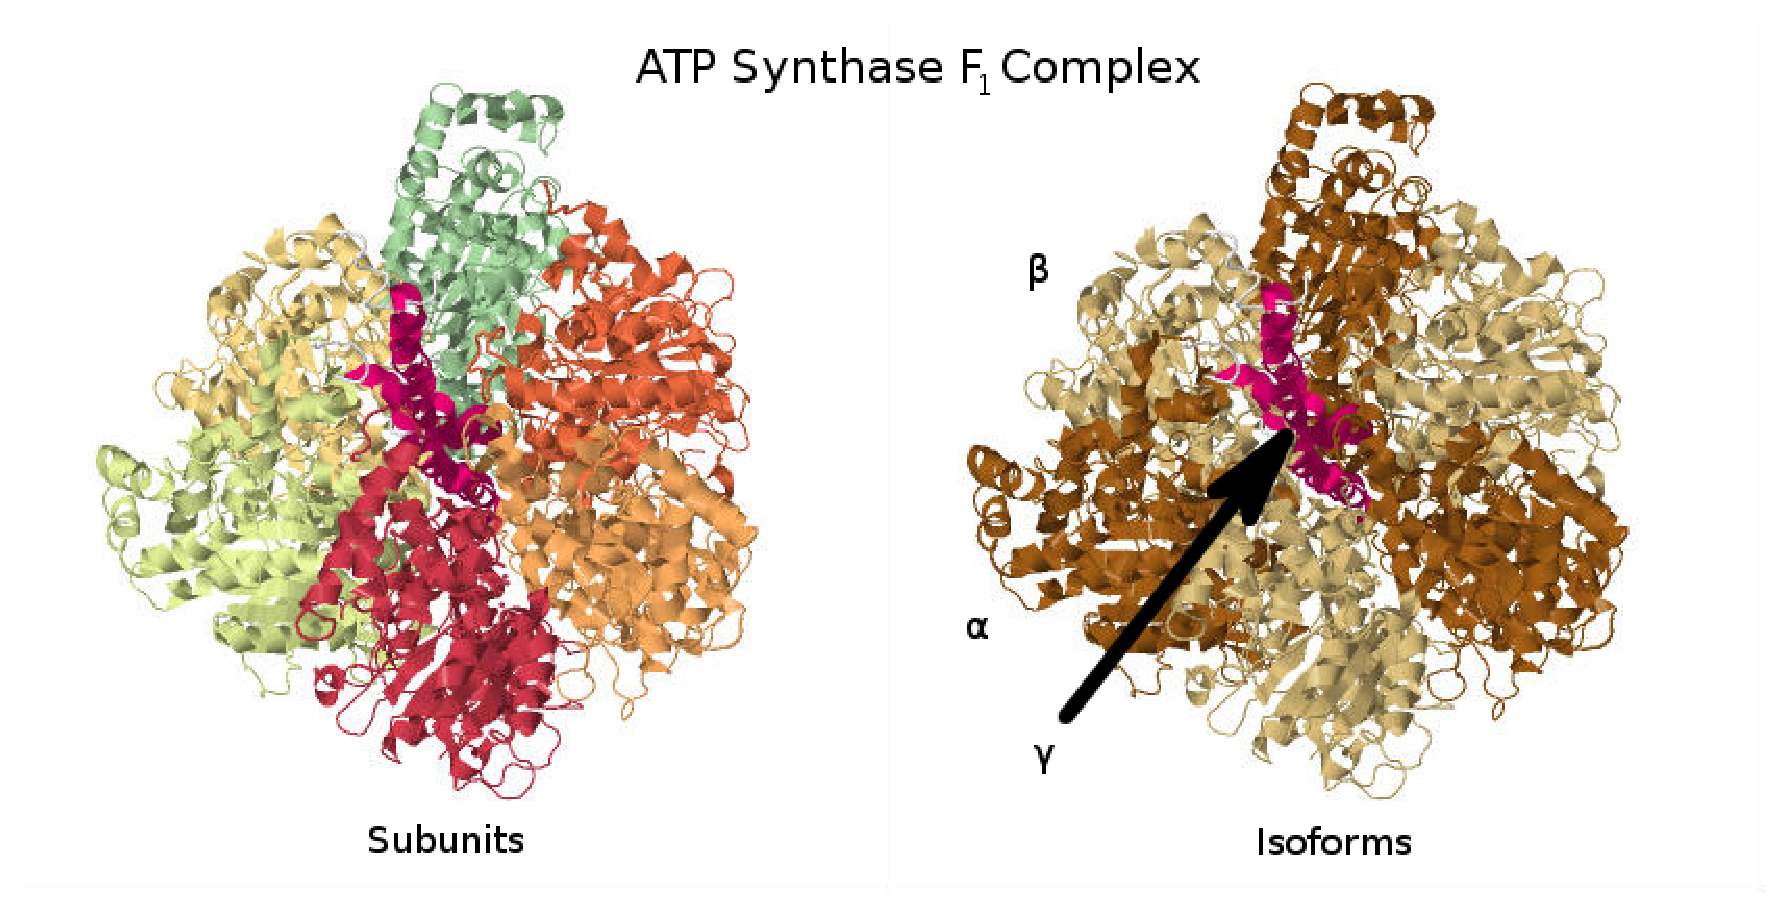
\includegraphics[clip=true,trim=0cm 0cm 0cm 0cm, width=12cm]{2F43}
\caption{Illustration of the $F_1$ part of the ATP Synthase complex
  (PDB ID 1E79; \citealt{Gibbons2000,Bernstein1978,Gezelter}).
  This illustration demonstrates both how an enzyme complex may be
  constituted by multiple subunits (left), and how some of those
  subunits may be products of the same gene and have differing
  stoichiometries within the complex (right).}
\end{figure*}

\emph{Assumption~\ref{asm:hierarchy}.}

The modeling of enzyme complex copy number can be tackled by using
nested sets of subcomplexes; each enzyme complex consists of multiple
subcomplexes, unlesss it is only a single protein or family of protein
isozymes.  These subcomplexes are required for the enzyme complex to
function (AND relationships), and can be thought of as the division of
the complex in to distinct units that each have some necessary
function for the complex, with the exception that we do not keep track
of the multiplicity of subcomplexes within a complex since this
information is, in the current state of affairs, not always known.
However, there may be alternative versions of each functional set
(given by OR relationships). Eventually, this nested embedding
terminates with a single protein or set of peptide isoforms
(e.g.\ isozymes).  In the case of ATP Synthase, one of its functional
sets is represented by the $F_1$ subcomplex. The $F_1$ subcomplex
itself can be viewed as having two immediate subcomplexes: the single
$\gamma$ (axle) subunit and three identical subcomplexes each made of
an $\alpha$ and $\beta$ subunit. Each $\alpha\beta$ pair works
together to bind ADP and catalyze the reaction \citep{Oster2003}. The
$\alpha\beta$ subcomplex itself then has two subcomplexes composed of
just an $\alpha$ subunit on the one hand and the $\beta$ subunit on
the other.  It is obvious that one of these base-level functional
subcomplexes (in this example, either $\gamma$ or $\alpha\beta$) will
be in most limited supply, and that it will best represent the overall
enzyme complex copy number (discounting the issues of multiplicity for
$\alpha\beta$, discussed above).

%
% Consider adding this as a Theorem/Proof:
%

The hierarhical structure just described, when written out in Boolean,
will give a rule in CNF (conjunctive normal form). This is because all
relations are ANDs (conjunctions), except possibly at the inner-most
subcomplexes that have alternative isoforms, which are expressed as
ORs (disjunctions). Since GPR rules alone only specify the
requirements for enzyme complex formation, we will see that not all
forms of boolean rules are equally useful in evaluating the enzyme
complex copy number, but we have established the assumptions in
Table~\ref{ECAssume} and an alternative and logically equivalent rule
\citep{Russell2009} under which we can estimate enzyme complex copy
number.


\def \ECAssumeCap {Assumptions in GPR-based Enzyme Complex Formation}
\label{ECAssume}
\ifthenelse{\boolean{thesisStyle}}{
  \begin{tabular}{| p{\textwidth} |}
  \hline
  \textbf{Table ~\ref{ECAssume}. \ECAssumeCap} \\
  \hline
  % I put this in to a separate file because formatting the table in different ways
% is difficult; it may even be better to have multiple versions of this table
% for different documents, but hopefully we can avoid such code duplication.

%Internal part of the table:

\begin{enumerate}
% This is really not related to GPR rules: 
%\ifthenelse{\boolean{thesisStyle}}{\item} {} \label{asm:mm}
%Fluxes in general strive to operate near the $V_{max}$ of the
%reaction, which is proportional to enzyme complex abundance.
\item \label{asm:expcorr}
Expression values are highly correlated with the copy numbers of their
corresponding peptide isoforms.
\item \label{asm:isozyme} 
Protein isoforms contributing to isozymes are considered part of the
same enzyme complex.
\item \label{asm:hierarchy}
Any enzyme complex can be described as a hierarchical subset of
(possibly redundant) subcomplexes; redundant subcomplexes, as
elaborated in (\ref{asm:nostoich}), are not currently modeled.
\item \label{asm:nostoich} 
Assume one copy of peptide per complex; exact isoform stoichiometry
is not considered.
\item \label{asm:sharing} 
With the exception of complexes having identical rules (i.e. the same
complex listed for different reactions), each copy of a peptide
is available for all complexes in the model.
\item \label{asm:active_site}
There is only one active site per enzyme complex.
\item \label{asm:enzyme_sensitivity} 
We assume that different pathways have similar flux sensitivities
with respect to their enzyme abundances.
\item \label{asm:holo} 
If a particular subcomplex can be catalyzed by A and it can also be
catalyzed by A and B (e.g. B acts as a regulatory unit, as in
holoenzymes), this just simplifies to A once expression values are
substituted in. Similarly, allosteric regulation is not
modeled. Relatedly, there are no NOT operations in GPR rules (just ANDs
and ORs).
\item \label{asm:chap} 
Enzyme complexes form without the assistance of protein chaperones and
formation is not coupled to other reactions.
\item \label{asm:posttrans}
Post-translational modifications do not affect complex formation.
\item \label{asm:rate} 
Rate of formation and degradation of complexes doesn't play a role,
since we assume steady-state. 
\end{enumerate}

  \\ \hline
  \end{tabular}

} {
  % For Bioinformatics:
  \begin{table*}[!t]
  \processtable{\ECAssumeCap \label{ECAssume}}{
  \begin{tabular}{| p{\textwidth} |}
  \hline
  % I put this in to a separate file because formatting the table in different ways
% is difficult; it may even be better to have multiple versions of this table
% for different documents, but hopefully we can avoid such code duplication.

%Internal part of the table:

\begin{enumerate}
% This is really not related to GPR rules: 
%\ifthenelse{\boolean{thesisStyle}}{\item} {} \label{asm:mm}
%Fluxes in general strive to operate near the $V_{max}$ of the
%reaction, which is proportional to enzyme complex abundance.
\item \label{asm:expcorr}
Expression values are highly correlated with the copy numbers of their
corresponding peptide isoforms.
\item \label{asm:isozyme} 
Protein isoforms contributing to isozymes are considered part of the
same enzyme complex.
\item \label{asm:hierarchy}
Any enzyme complex can be described as a hierarchical subset of
(possibly redundant) subcomplexes; redundant subcomplexes, as
elaborated in (\ref{asm:nostoich}), are not currently modeled.
\item \label{asm:nostoich} 
Assume one copy of peptide per complex; exact isoform stoichiometry
is not considered.
\item \label{asm:sharing} 
With the exception of complexes having identical rules (i.e. the same
complex listed for different reactions), each copy of a peptide
is available for all complexes in the model.
\item \label{asm:active_site}
There is only one active site per enzyme complex.
\item \label{asm:enzyme_sensitivity} 
We assume that different pathways have similar flux sensitivities
with respect to their enzyme abundances.
\item \label{asm:holo} 
If a particular subcomplex can be catalyzed by A and it can also be
catalyzed by A and B (e.g. B acts as a regulatory unit, as in
holoenzymes), this just simplifies to A once expression values are
substituted in. Similarly, allosteric regulation is not
modeled. Relatedly, there are no NOT operations in GPR rules (just ANDs
and ORs).
\item \label{asm:chap} 
Enzyme complexes form without the assistance of protein chaperones and
formation is not coupled to other reactions.
\item \label{asm:posttrans}
Post-translational modifications do not affect complex formation.
\item \label{asm:rate} 
Rate of formation and degradation of complexes doesn't play a role,
since we assume steady-state. 
\end{enumerate}

  \\ \hline
  \end{tabular}
  }
  {} % caption
  \end{table*}
}

There is no guarantee that a GPR rule has been written down with this
hierarchical structure in mind, though it is likely the case much of
the time as it is a natural way to model complexes.  However, any GPR
rule can be interpreted in the context of this hierarchical view due
to the existence of a logically equivlaent CNF rule for any non-CNF
rule, and it is obvious that logical equivalence is all that is
required to check for enzyme complex formation when exact isoform
stoichiometry is unknown.  As an example, we consider another common
formulation for GPRs, and a way to think about enzyme
structure---disjunctive normal form (DNF).  A DNF rule is a
disjunctive list of conjunctions of peptide isoforms, where each
conjunction is some variation of the enzyme complex due to
substituting in different isoforms for some of the required
subunits. A rule with a more complicated structure and compatible
isoforms across subcomplexes may be written more succinctinly in CNF,
whereas a rule with only very few alternatives derived from isoform
variants may be reprsented clearly with DNF.  In rare cases, it is
possible that a GPR rule is written in neither DNF or CNF, perhaps
because neither of these two alternatives above are stricly the case,
and some other rule is more succinct.

\emph{Assumptions~\ref{asm:nostoich},~\ref{asm:sharing}~and~\ref{asm:active_site}.}
One active site per enzyme complex implies a single complex can only
catalyze one reaction at a time. Multimeric complexes with one active
site per identical subunit would be considered as one enzyme complex
per subunit in this model.  Note that it is possible for an enzyme
complex to catalyze different reactions. In fact, some transporter
complexes can transfer many different metabolites \hl{across a lipid
  bilayer---up to X in the case of Y}. Another example is the ligation or hydrolysis of
nucleotide, fatty acid, or peptide chains, where chains of different
length may all be substrates or products of the same enzyme
complex. While we do not explicitly consider these in
Algorithm~\ref{alg:ReductionToCNF}, these redundancies are taken into
account subsequently in Algorithm~\ref{alg:FALCON}.

What is currently not considered in our process is that some peptide
isoforms may find use in completely different complexes, and in some
cases, individual peptides may have multiple active sites; in the
first case, we assume an unrealistic case of superposition where the
isoform can simultaneously function in more than one complex. The
primary reason we have not tackled this problem is because exact
subunit stoichiometry of most enzyme complexes is not accurately
known, but an increasing abundance of data on BRENDA
\citep{Schomburg2013} gives some hope to this problem. A recent
\textit{E. coli} metabolic model incorporating the metabolism of all
known gene products \citep{O'Brien2013} also includes putative
enzyme complex stoichiometry in GPRs. For the second point, there
are a few enzymes where a single polpeptide may have multiple active
sites (e.g.\ fatty acid synthase), and this is not currently taken into
account in our model.

\emph{Assumption~\ref{asm:holo}.}
We do not make any special assumptions requiring symmetry of an
isoform within a complex. For instance, the example in
assumption~\ref{asm:holo} shows how you might have one subcomponent
composed of a single isoform, and another subcomponent composed of
that gene in addition to another isoform. In this case, it is simply
reduced to being the first gene only that is required, since clearly
the second is strictly optional. That isn't to say that the second
gene may not have some effect, such as (potentially) aiding in
structural ability or altering the catalytic rate, but it should have
no bearing on the formation of a functional catalytic
complex. Holoenzymes---enzymes with metabolic cofactors or protein
subunits that have a regulatory function for the complex---would
likely be the only situation where this type of rule might need to be
considered in more detail. But in the absence of detailed kinetic
information, this consideration (much like allosteric
regulation) is not useful.

\emph{Assumptions~\ref{asm:chap}~and~\ref{asm:rate}.}
Due to the quickness, stability, and energetic favorability of enzyme
complex formation, the absence of chaperones or coupled metabolic
reactions required for complex formation may be reasonable
assumptions, but further research is warranted \citep{Karr2012}.
Additionally, as in metabolism, we assume a steady state for complex
formation, so that rate laws regarding complex formation aren't
needed. However, further research may be warranted to investigate the
use of a penalty for complex levels based on mass action and
protein-docking information. Requisite to this would be addressing
assumption~\ref{asm:nostoich}. It would be surprising (but not
impossible) if such a penalty were very larege due to the cost this
would imply for many of the large and important enzyme complexes
present in all organisms \citep{Nelson2008}.

\section{Proof for the minDisjunction algorithm}

Although the logic in the main text may be straightforward, we show
here in more verbosity that Algorithm~\ref{alg:ReductionToCNF} works
as described.

\begin{Theorem}
\label{thm:ReductionToCNF}
Algorithm~\ref{alg:ReductionToCNF} returns the disjunction with
minimum expression value among all disjunctions of a rule in CNF.
\end{Theorem}

\begin{proof}
The third step in the while-loop does not affect the
underlying logic, so we only need to consider the effect of step one
on step two.  Let us first consider when expressions $x_1, ..., x_4$
are all literals in step two to cover the most complex case, and that
$x_i^{(e)}$ denotes the expression measurement for gene $x_i$. Assume
WLOG that $x_1 \lor x_3$ attains the minimum expression among the
disjunctions. Then we have:

\begin{align*}
&x_{1}^{(e)} + x_{3}^{(e)} \leq x_{1}^{(e)} + x_{4}^{(e)} \Rightarrow x_{3}^{(e)} \leq x_{4}^{(e)} \\
&x_{1}^{(e)} + x_{3}^{(e)} \leq x_{2}^{(e)} + x_{3}^{(e)} \Rightarrow x_{1}^{(e)} \leq x_{2}^{(e)} 
\end{align*}

Applying this result in conjunction to step one in the while-loop to
the original expression, $(x_1 \land x_2) \lor (x_3 \land x_4)$, we
immediately arrive at $(x_1) \lor (x_3)$, which gives our originally
assumed minimum. To show that this result doesn't depend on the $x_i$
being literals, merely consider repeating this process recursively for
each $x_i$ that is not a literal to arrive at two different
evaluations for $x_i^{(e)}$ (one where each evaluation is done with
reduction, and one where we evaluate entirely without reduction).
Since the process cannot continue indefinitely, eventually there is a
base case involving only literals, and the above result shows that, at
each step, as we backtrack from the base case, both evaluations will
be identical. The desired result is obtained because
Algorithm~\ref{alg:ReductionToCNF} without step one simply yields CNF,
and it follows that adding step one will yield the disjunction with
minimum expression value of the rule in CNF.
\end{proof}

\section{Code excerpt for minimum disjunction algorithm}
\label{sec:code}

The following code is written in ATS, a type-safe language including
syntax similar to SML while having direct access to C types
\citep{ATStypes03}. \texttt{GREXP} describes a datatype that is used
for storing the parse trees of Boolean rules (without negation).  A
\texttt{GREXP} can then be manipulated by the function \texttt{toCNF}
to be converted to a conjunctive normal form. We make use of the
reduction rule mentioned previously by calling the \texttt{minConj}
function. The \texttt{conjunctivize} function is a helper function to
deal with different structures for \texttt{GRconj} and \texttt{GRdisj}
(one is set based, one is parse-tree based; note this described in the
data(view)type defintion). We note that this is a recursive,
functional implementation of Algorithm~\ref{alg:ReductionToCNF}, which
seems more straightforward than a procedural implementation.

\begin{verbatim}
dataviewtype GREXP = 
  | GRgenes of genes
  | GRconj of genes
  | GRconj of (GREXP,GREXP)
  | GRdisj of genes
  | GRdisj of (GREXP,GREXP)

extern
fun toCNF (bexp: GREXP, emap: &gDMap): GREXP

implement
toCNF (bexp, emap): GREXP = let     
  val LR:GREXP = (case+ bexp of 
    | ~GRconj(ex1,ex2) => GRconj (toCNF(ex1,emap),toCNF(ex2,emap))
    | ~GRdisj(ex1,ex2) => GRdisj (toCNF(ex1,emap),toCNF(ex2,emap))   
    | GR => GR):GREXP
  in (case+ LR of  
    | ~GRconj(ex1,ex2) => minConj(GRconj(ex1,ex2),emap) 
    | ~GRdisj(ex1,ex2) => (case+ (ex1,ex2) of
      // Handle disjunctive leaf cases:         
      | (~GRdisj(lx), ~GRgenes(g)) => GRdisj (lx + g) 
      | (~GRgenes(g), ~GRdisj(rx)) => GRdisj (rx + g)
      | (~GRdisj(lx), ~GRdisj(rx)) => GRdisj (lx + rx)
      | (~GRgenes(g1), ~GRgenes(g2)) => GRdisj (g1 + g2)

      // Distribute OR over ANDs:
      | (~GRconj(x1,x2), ~GRconj(g)) => conj1(x1,x2,g,emap) 
      | (~GRconj(g), ~GRconj(x1,x2)) => conj1(x1,x2,g,emap) 
      | (~GRconj(g1), ~GRconj(g2)) => conj2(g1,g2,emap)
      | (~GRconj(lx1,lx2), ~GRconj(rx1,rx2)) => let
        val lx1c = GREXP_copy(lx1)
        val lx2c = GREXP_copy(lx2) 
        val rx1c = GREXP_copy(rx1)
        val rx2c = GREXP_copy(rx2) 
        in GRconj(GRconj(GRconj(toCNF(GRdisj(lx1,rx1),emap), 
          toCNF(GRdisj (lx2, rx1c ),emap)),
          toCNF(GRdisj (lx1c, rx2),emap)), 
          toCNF(GRdisj (lx2c, rx2c),emap)) 
        end

      // Handle e.g.: (.. OR ..) OR (.. AND ...) 
      | (~GRconj(lx1,lx2), RX) => let
        val RXc = GREXP_copy(RX)
        in GRconj(toCNF(GRdisj(lx1,RX),emap),
          toCNF(GRdisj(lx2,RXc),emap)) 
        end
      | (LX ,~GRconj(rx1,rx2)) => let
        val LXc = GREXP_copy(LX)
        in GRconj(toCNF(GRdisj(LX,rx1),emap),
          toCNF(GRdisj(LXc,rx2),emap)) 
        end
      | (~GRconj(gc), RX) => let
        val retGR = toCNF(conjunctivize(RX, gc,emap),emap)
        val _ = genes_free(gc)
        in retGR end
      | (LX, ~GRconj(gc)) => let
        val retGR = toCNF (conjunctivize(LX, gc,emap),emap)
        val _ = genes_free(gc)
        in retGR end
      // All other disjunctive cases
      | (_,_) => GRdisj(toCNF(ex1,emap),toCNF(ex2,emap))
      ):GREXP
    | EX => EX
    ):GREXP
  end
\end{verbatim}

\section{FALCON internals and experimental features}
\label{sec:internals}

\subsection{EXPCON: expression constraints for $V_{max}$}
An experimental feature that has been implemented is to constrain
enzymatic fluxes to be strictly less than or equal to the
automatically scaled enzyme abundance. For example, in the
notation of Algorithm~\ref{alg:FALCON}, for each reversible $v_j$
associated to enzyme complex $i$, we would have the additional
constraints:

\[ v_{j,f} \leq n e_i \]
\[ v_{j,b} \leq n e_i \]

This feature may be employed by setting the \texttt{EXPCON} parameter
to \texttt{true} when calling \texttt{falcon}. We implemented this
feature because we have seen and heard of others seeing promising
results when na\"ively using scaled expression to act as a surrogate for
$V_{max}$ in standard FBA (for an abstraction and example, see
\citealt{Colijn2009}). In the present study, we observed similar
results when using this parameter, suggesting that---at least for the
yeast models---this parameter may provide additional benefit when
appended to the existing FALCON machinery. We speculate that larger
and less constrained models may benefit from employing this parameter.

\subsection{Regularization}
Although sometimes called by different names, regularization is an
optimization technique that alters a problem so that there is some
penalty for variables taking on large values, where large may be
defined in different ways. In our case, since we are using a linear
programming problem, it is most convenient to use the $L_1$-norm to
assess how large a penalty should be given. We employ this as an
optional parameter to \texttt{falcon}, \texttt{rc} that is applied to
all flux values.  Regularization has been found to be a biologically
important objective in microbes \citep{Schuetz2012}, but we didn't
find any significant differences when using it in the present study.

\subsection{Growth rates}
Sometimes a growth rate may be known or we may wish to simulate a
growth rate. If we have a high-confidence biomass pseudo-reaction in
our model, the optional \texttt{minFit} parameter to \texttt{falcon}
can be used to set the minimum growth rate. Since biomass is a
complicated sink in the model, it is apparentl unlikely that the
FALCON objective will direct flux into biomass directly, so other
measures of growth rate may also be warranted, such as accounting
for individual sink reactions. This part of \texttt{falcon} could
easily be modified to support more reactions beyond biomass.

\subsection{Debugging and developing falcon}
The \texttt{FDEBUG} parameter to \texttt{falcon} can be used to
display additional information while the FALCON algorithm is
running. As this can potentially be quite verbose, \texttt{FDEBUG} is
normally set to \texttt{false}. \texttt{FDEBUG} is also a parameter to
\texttt{computeMinDisj}, the MATLAB wrapper function for the
\texttt{minDisj} executable, and is used similarly there.


\subsection{Including reversible reactions in the FALCON objective}
Since FALCON has been designed for use with irreversible models, there
is no mathematical problem with including both the forward and
backward reactions of a reversible reaction in the FALCON objective,
but this may give undesired results in some cases, such as cycles
between the forward and backward reactions (the cycles are not a
problem directly because they can be removed: see the functions
\texttt{setFBRxnDirection} in \texttt{falcom.m}.  These cycles can
then give rise to objective values that may be quite high simply due
to having many cycles.

%\subsection{Linear Fractional Program (Charnes-Cooper) Transformation}
%Since our denominator is simply the variable $n$, it is always
%required to be equal to 1 in the transformed problem. However,
%this is scaled by $z$, which may vary. To be sure that $z$ never
%goes to zero, we set a lower about on $z$ with the \texttt{ZMIN}
%variable. We know $z = 0$ is undesirable in our case since
%we have $z = \frac{1}{n}$ and $v_original = n v_{LFP} = \frac{v_{LFP}}{z}$.
%!! Actually, we should not need this, since dividing by small z would make for 
% a very large original objective value. This may only be needed in cases
% where we aren't using a true LFP.

\subsection{LP solver settings}
We have exclusively used the Gurobi solver \citep{gurobi} for this
work, which is a highly competitive solver that employs by default a
parallel strategy to solving problems: a different algorithm is run
simultaneously, and as soon as one algorithm finished the others
terminate. Of course, if there is a clear choice of algorithm for a
particular problem class, this should be used in production settings
to avoid wasted CPU time and memory. As we see in Table~\ref{xx}, the
dual-simplex method is best for time-efficiency. The dual-simplex
method is also recommended for memory-efficiency by Gurobi
documentation, but we did not observe any differences in memory for
different solver methods..

In our case, we had the following results for Yeast 5 (with minimal
directionality constraints) and an expanded
Recon 2.1 \hl{cites} (to use relatively small and very large models):

%Insert table here.
\begin{center}
\begin{tabular}{rrrr}
\emph{Model}               & \emph{Primal-Simplex} & \emph{Dual-Simplex} & \emph{Barrier} \\
Yeast5 (2061 reactions)    & $7.4088 \pm 0.0171  $ & $7.9991 \pm 0.0171$ & $7.3267 \pm 0.0116$ \\ 
Yeast7 (3498 reactions)    & $ $ & $72.4839 \pm 0.0430       $ & $51.7103 \pm 1.5659$ \\
Recon 2.1 (xx reactions)   & $ $ & $ $ & \\
\end{tabular}
\end{center}

The time for completion of Yeast7 with the primal-simplex solver is
less because fewer iterations were completed before the solver failed
to find a feasible solution; we verified that this is a numeric issue
in Gurobi and can be fixed by setting the Gurobi parameter
\texttt{MarkowitzTol} to a larger value (which decreases
time-efficiency but limits the numerical error in the
simplex algorithm) and by substituting a less tight constraint in the
update to $V_{lb}^{\Sigma}$ (the \texttt{flux\_sum} variable in
\texttt{falcon}). In practice, failure for the algorithm to converge
at an advanced iteration is rare and is not always a major problem (since the previous
flux estimate by the advanced iteration should already be quite good), but it
is certainly undesirable; a warning message will be printed by
\texttt{falcon} if this occurs, at which point parameter settings can
be investigated. In the future, we plan to improve \texttt{falcon} so
that parameters will be adjusted as neeeded during progression of the
algorithm after finding a good test suite of models and data. For now,
we use the dual-simplex solver, for which \hl{we have always had good}
results.

Because the number of iterations depends non-trivially on the model
and the expression data, it may be more helfpul to look at the 
average time per iteration in the above examples.

\begin{center}
\begin{tabular}{rrrr}
\emph{Model}               & \emph{Primal-Simplex} & \emph{Dual-Simplex} & \emph{Barrier} \\
Yeast5 (2061 reactions)    & $ $ & $ $ & $ $ \\ 
Yeast7 (3498 reactions)    & $ $ & $ $ & $ $ \\
Recon 2.1 (xx reactions)   & $ $ & $ $ & $ $ \\
\end{tabular}
\end{center}


It is not possible to pass the Gurobi \texttt{method} parameter to
\texttt{gurboi} in the COBRA Toolbox by default, but to keep our code
as close as possible to the COBRA Toolbox API, we have copied
\texttt{solveCobraLP.m} to the file \texttt{solveFalconLP.m} and
modified it to use the optimal method parameters. Other parameters
could also be passed easily. \texttt{solveFalconLP} is only called if
\texttt{gurobi} is detected as a MATLAB executable (MEX) file;
otherwise the default solver specified for the COBRA Toolbox will be
used. At the time of this release, \texttt{solveFalconLP} should be
completely compatible with all other possible calls made to
\texttt{solveCobraLP}, so in principle the latter could be replaced,
but it is not reccommended in case the COBRA Toolbox API changes. If a
user wishes to use some solver other than Gurobi, it should be easy to
alter \texttt{solveFalconLP.m} and \texttt{falcon.m} to support custom
parameters. 

\section{Generation of figures and tables}

\subsection{Minimally constrained yeast models}
The MATLAB function \texttt{removeEnzymeIrrevs} was written to find
all enzymatic reactions in a model that are annotated as reversible
but are constrained to operate in one direction only. The script then
changes the bounds to allow flux in both directions. The fuction
\texttt{useYN5irrevs} copies the irreversible annotations found in
Yeast 5.21 \citep{Lee2012} to a newer yeast model, but could in
principle be used for any two models; by default, this script is coded
to first call \texttt{removeEnzymeIrrevs} on both models before
copying irreversible annotations. To change this setting so that
\texttt{removeEnzymeIrrevs} is not applied to either model, set the
\texttt{noDir} argument.

\subsection{Expression perturbation analysis}
\hl{Describe log-normal noise sampling here first.}
    %
%                          %
%%%%%%%%%%%%%%%%%%%%%%%%%%%%

\bibliography{dissertation}

\end{document}
